% =============================================================================
% Spark Match - Copiloto de Orientacion Vocacional con IA Generativa
% Trabajo de Fin de Programa - II Programa de Especializacion en IA Generativa
% y Machine Learning Ops - Universidad Nacional de Ingenieria (UNI)
% =============================================================================

% =============================================================================
% Preamble - Paquetes y configuracion global
% Articulo: Spark Match - Copiloto de Orientacion Vocacional con IA Generativa
% =============================================================================

\documentclass[12pt, a4paper]{article}

% --- Codificacion y lenguaje ---
\usepackage[utf8]{inputenc}
\usepackage[T1]{fontenc}
\usepackage[spanish]{babel}

% --- Geometria de pagina ---
\usepackage[top=2.5cm, bottom=2.5cm, left=3cm, right=2.5cm]{geometry}

% --- Tipografia ---
\usepackage{lmodern}

% --- Graficos e imagenes ---
\usepackage{graphicx}
\graphicspath{{figures/}}
\usepackage{float}
\usepackage[font=small, labelfont=bf]{caption}
\usepackage{subcaption}

% --- Tablas ---
\usepackage{booktabs}
\usepackage{array}
\usepackage{tabularx}
\usepackage{multirow}

% --- Listas ---
\usepackage{enumitem}

% --- Matematicas ---
\usepackage{amsmath}
\usepackage{amssymb}

% --- Colores y enlaces ---
\usepackage{xcolor}
\PassOptionsToPackage{hyphens}{url} % permitir cortar URLs en los guiones
\usepackage[colorlinks=true, linkcolor=black, citecolor=blue, urlcolor=blue]{hyperref}
\usepackage{url}
\urlstyle{same}
% Permitir que las URLs largas partan en guiones y barras (evita que se salgan de las cajas)
\Urlmuskip=0mu plus 1mu\relax

% --- Codigo fuente ---
\usepackage{listings}

\definecolor{codegreen}{rgb}{0.0, 0.5, 0.0}
\definecolor{codegray}{rgb}{0.5, 0.5, 0.5}
\definecolor{codepurple}{rgb}{0.58, 0.0, 0.82}
\definecolor{codeblue}{rgb}{0.0, 0.0, 0.7}
\definecolor{codeorange}{rgb}{0.95, 0.50, 0.10}
\definecolor{backcolour}{rgb}{0.97, 0.97, 0.97}

\lstdefinestyle{pythonstyle}{
    backgroundcolor=\color{backcolour},
    commentstyle=\color{codegreen}\itshape,
    keywordstyle=\color{codeblue}\bfseries,
    numberstyle=\tiny\color{codegray},
    stringstyle=\color{codepurple},
    basicstyle=\ttfamily\small,
    breakatwhitespace=false,
    breaklines=true,
    captionpos=b,
    keepspaces=true,
    numbers=left,
    numbersep=8pt,
    showspaces=false,
    showstringspaces=false,
    showtabs=false,
    tabsize=4,
    frame=single,
    rulecolor=\color{codegray},
    framesep=5pt,
    xleftmargin=15pt,
    framexleftmargin=15pt
}

\lstdefinestyle{bashstyle}{
    backgroundcolor=\color{backcolour},
    basicstyle=\ttfamily\small,
    breaklines=true,
    captionpos=b,
    frame=single,
    rulecolor=\color{codegray},
    numbers=none,
    xleftmargin=10pt,
    framexleftmargin=10pt,
    aboveskip=10pt,
    belowskip=10pt
}

\lstdefinestyle{yamlstyle}{
    backgroundcolor=\color{backcolour},
    commentstyle=\color{codegreen}\itshape,
    keywordstyle=\color{codeorange}\bfseries,
    basicstyle=\ttfamily\small,
    breaklines=true,
    captionpos=b,
    frame=single,
    rulecolor=\color{codegray},
    numbers=none,
    xleftmargin=10pt,
    framexleftmargin=10pt
}

\lstdefinestyle{jsonstyle}{
    backgroundcolor=\color{backcolour},
    basicstyle=\ttfamily\small,
    breaklines=true,
    captionpos=b,
    frame=single,
    rulecolor=\color{codegray},
    numbers=none,
    xleftmargin=10pt,
    framexleftmargin=10pt
}

\lstset{
    style=pythonstyle,
    language=Python,
    float=H,
    aboveskip=10pt,
    belowskip=10pt,
    literate=
        {\'a}{{\'a}}1 {\'e}{{\'e}}1 {\'i}{{\'i}}1 {\'o}{{\'o}}1 {\'u}{{\'u}}1
        {\'A}{{\'A}}1 {\'E}{{\'E}}1 {\'I}{{\'I}}1 {\'O}{{\'O}}1 {\'U}{{\'U}}1
        {\~n}{{\~n}}1 {\~N}{{\~N}}1
}

% --- Algoritmos (pseudocodigo con algorithmic) ---
\usepackage{algorithm}
\usepackage{algorithmic}

% --- TikZ para diagramas ---
\usepackage{tikz}
\usetikzlibrary{arrows.meta, positioning, calc, shapes.geometric, fit, backgrounds, babel}

% --- Encabezados y pies de pagina ---
\usepackage{fancyhdr}
\setlength{\headheight}{14pt}
\pagestyle{fancy}
\fancyhf{}
\fancyhead[L]{\small Spark Match - TFP UNI}
\fancyhead[R]{\small IA Generativa y MLOps}
\fancyfoot[C]{\thepage}
\renewcommand{\headrulewidth}{0.4pt}
\renewcommand{\footrulewidth}{0pt}

% --- Espaciado ---
\usepackage{setspace}
\onehalfspacing
\setlength{\parskip}{6pt}
\setlength{\parindent}{0pt}

% --- Bibliografia ---
\usepackage[numbers, sort&compress]{natbib}
\setlength{\bibsep}{4pt}

% --- Cajas para repositorios ---
\usepackage{tcolorbox}
\tcbuselibrary{breakable}

\begin{document}

% --- Portada ---
\begin{titlepage}
    \centering
    \vspace*{1.5cm}

    \rule{\linewidth}{0.5pt}\\[0.4cm]
    {\Large \textbf{Universidad Nacional de Ingenier\'ia}}\\[0.2cm]
    {\large Facultad de Ingenier\'ia Econ\'omica, Estad\'istica y Ciencias Sociales}\\[0.1cm]
    {\normalsize Centro de Formaci\'on Continua}\\[0.1cm]
    {\normalsize II Programa de Especializaci\'on en IA Generativa y Machine Learning Ops}\\
    \rule{\linewidth}{0.5pt}\\[2cm]

    {\LARGE \textbf{Spark Match}}\\[0.5cm]
    {\Large Copiloto Inteligente para la Elecci\'on de Carrera Profesional\\basado en IA Generativa y Recomendaci\'on H\'ibrida}\\[1cm]
    {\normalsize Trabajo de Fin de Programa: dise\~no, implementaci\'on, despliegue y evaluaci\'on\\
    de un sistema de orientaci\'on vocacional con agentes LLM y MLOps en AWS}\\[3cm]

    \begin{tabular}{rl}
        \textbf{Docente:}      & [Nombre del Docente] \\[0.3cm]
        \textbf{Integrantes:}  & Fabiola G. Tapara Quispe \\
                                & Angel E. Hincho Jove \\
                                & Andy B. Huamani Tacoma \\
                                & Nikolai A. Asencios Garc\'ia \\
                                & David Barreto Lara \\[0.3cm]
        \textbf{Programa:}     & II Programa de Especializaci\'on en IA Generativa y MLOps \\[0.3cm]
        \textbf{Ciclo:}        & 2026-I \\[0.3cm]
        \textbf{Fecha:}        & 09 de agosto de 2026 \\
    \end{tabular}

    \vfill

    \rule{\linewidth}{0.5pt}\\[0.2cm]
    {\small Lima, Per\'u --- 2026}
\end{titlepage}

% --- Tabla de contenidos ---
\tableofcontents
\newpage

% --- Resumen ---
\section*{Resumen}

Spark Match (CareerMatch Per\'u) es un asistente conversacional basado en IA
generativa que orienta a estudiantes y padres de familia en la elecci\'on de
carrera y universidad en el Per\'u. El sistema combina un agente de lenguaje
(un LLM \emph{Claude}, servido mediante \emph{AWS Bedrock}), que interpreta en
lenguaje natural las preferencias del estudiante y luego explica los resultados,
con un motor de recomendaci\'on transparente en Python que asigna un puntaje a
cada combinaci\'on carrera--universidad usando datos oficiales del portal
\emph{Ponte en Carrera} (MINEDU). A diferencia de los sistemas con pesos fijos,
los pesos de cada criterio son inferidos din\'amicamente por el LLM a partir de la
conversaci\'on, y la afinidad vocacional se modela con el esquema RIASEC de
Holland. La plataforma se apoya en un backend \emph{serverless} en TypeScript
(AWS Lambda + EventBridge + SAM), un frontend en Angular y un agente en Python
(LangGraph). El proyecto incorpora pr\'acticas de MLOps mediante el versionado de
prompts, f\'ormula de scoring y datos, la observabilidad del agente con LangSmith,
el seguimiento de experimentos con Weights \& Biases y CI/CD e infraestructura
como c\'odigo (Terraform) sobre AWS. Este documento presenta el caso de uso, la
selecci\'on de modelo y datos, la ingenier\'ia de prompts, la arquitectura, el
prototipo, la evaluaci\'on y las recomendaciones.

\vspace{0.5cm}
\noindent\textbf{Palabras clave:} orientaci\'on vocacional, sistemas de recomendaci\'on, IA generativa, LLM, agentes, RIASEC, MLOps, AWS Bedrock, serverless, LangSmith.

\newpage

% --- Repositorios del proyecto ---
\begin{tcolorbox}[title=Repositorios y recursos del proyecto, breakable, colback=blue!2, colframe=blue!40!black]
\renewcommand{\arraystretch}{1.4}
\begin{tabularx}{\linewidth}{@{} >{\bfseries}l >{\raggedright\arraybackslash}X @{}}
    Organizaci\'on & \url{https://github.com/spark-match} \\
    DevOps (CI/CD) & \url{https://github.com/spark-match/spark-match-01-devops} \\
    Infraestructura (Terraform/AWS) & \url{https://github.com/spark-match/spark-match-02-infrastructure} \\
    Backend (Serverless TypeScript) & \url{https://github.com/spark-match/spark-match-03-backend} \\
    Frontend (Angular) & \url{https://github.com/spark-match/spark-match-04-frontend} \\
    Pipeline de Datos & \url{https://github.com/spark-match/spark-match-05-data-pipeline} \\
    Entrenamiento de Modelos & \url{https://github.com/spark-match/spark-match-06-model-training} \\
    Este art\'iculo (LaTeX) & \url{https://github.com/spark-match/spark-match-07-article} \\
    Agente conversacional (Deep Agent) & \url{https://github.com/spark-match/spark-match-08-deep-agent} \\
\end{tabularx}
\end{tcolorbox}

% --- Secciones ---
% ============================================================================
% Seccion 1: Descripcion del Caso de Uso
% TFP - Rubrica: 1 punto
% ============================================================================
\section{Descripci\'on del caso de uso}

% TODO: Contextualizar el problema de orientacion vocacional en Peru.
% Citar fuentes oficiales (INEI, MINEDU, SUNEDU) sobre oferta educativa,
% tasas de desercion, dificultad de acceso a informacion comparada.

% TODO: Justificar por que IA Generativa + MLOps es adecuado para este caso
% (razonamiento conversacional, recomendaciones personalizadas, reproducibilidad).

% TODO: Definir objetivo de negocio (orientar mejor al estudiante) y objetivo
% tecnico (asistente conversacional hibrido LLM + scoring determinista).

Los estudiantes preuniversitarios en el Per\'u enfrentan una dificultad significativa al momento de elegir una carrera profesional y la instituci\'on de educaci\'on superior donde cursarla. La informaci\'on oficial --- salarios de los egresados, costos de matr\'icula, tasas de admisi\'on, ubicaci\'on de sedes, modalidades de ingreso --- se encuentra dispersa en m\'ultiples portales institucionales y es dif\'icil de comparar de manera sistem\'atica.

[Motivacion del proyecto: por que un copiloto conversacional resuelve este problema mejor que las evaluaciones vocacionales estaticas tradicionales.]

\subsection{Problem\'atica del negocio}

[Describir la problematica concreta con datos. Ejemplos:
- Fragmentacion de la informacion oficial (SUNEDU, portales universitarios).
- Evaluaciones vocacionales estaticas que no consideran restricciones reales (presupuesto, geografia).
- Falta de explicabilidad en recomendaciones automatizadas.]

\subsection{Objetivo de negocio}

[Que decision del usuario queremos mejorar. Ej: reducir el tiempo promedio de decision vocacional, aumentar la satisfaccion con la carrera elegida, etc.]

\subsection{Objetivo t\'ecnico}

[Construir un sistema que:
- Interprete lenguaje natural del estudiante (filtros + chat libre).
- Genere pesos din'amicos para un motor de scoring determinista.
- Devuelva un ranking Top-N de combinaciones Carrera-Universidad con justificacion en lenguaje natural.
- Sea reproducible, versionado y desplegado en AWS.]

\subsection{Fuentes de relevancia}

[Listar fuentes que respalden la relevancia del caso. Ej: estudios de desercion universitaria, reportes de SUNEDU sobre la oferta educativa, papers sobre sistemas de recomendacion en educacion (EdTech).]
% ============================================================================
% Seccion 2: Seleccion de Modelo y Datos
% TFP - Rubrica: 1 punto
% ============================================================================
\section{Selecci\'on de modelo y datos}

% TODO: Documentar el LLM elegido (Gemini API / AWS Bedrock), arquitectura,
% parametros, costos por token y motivo de la eleccion frente a alternativas
% (OpenAI GPT, Anthropic Claude, Llama 3, Mistral).

% TODO: Describir el dataset: fuente (SUNEDU, portales institucionales),
% volumen, esquema de columnas (carrera, universidad, region, costo,
% salario esperado, tasa de admision), periodo de recoleccion.

% TODO: Documentar pipeline de preprocesamiento: limpieza, normalizacion,
% imputacion de nulos, escalado, generacion de embeddings si aplica.

\subsection{Modelo generativo / fundacional}

[Describir el LLM elegido:
- Proveedor: AWS Bedrock (MaaS) o Google Gemini API [definir].
- Modelo especifico: Claude 3 / Llama 3 / Titan / Gemini Pro [definir].
- Justificacion frente a alternativas (latencia, costo, ventana de contexto, soporte en espa\~nol).
- Parametros: \texttt{temperature}, \texttt{top\_p}, \texttt{max\_tokens}, system prompt base.]

\subsection{Dataset}

[Caracterizar el dataset:
- Fuente: scrapeo con Selenium de portales SUNEDU + ministerios + universidades.
- Volumen: numero de universidades, carreras, registros por region.
- Esquema: columnas del CSV normalizado.
- Periodo de recoleccion: a\~no/semestre.
- Almacenamiento: DVC remoto (S3) + versionado.]

\subsection{Preprocesamiento y embeddings}

[Pipeline de datos documentado paso a paso:
- Limpieza (duplicados, outliers).
- Imputacion de nulos (mediana, KNN, modelo).
- Normalizacion / escalado (MinMax, StandardScaler).
- Generacion de embeddings (si aplica: Sentence-Transformers para descripciones de carreras).
- Versionado con DVC.]

\begin{lstlisting}[style=pythonstyle, caption={Ejemplo: carga del dataset versionado con DVC}, label={lst:dvc-load}]
import dvc.api
import pandas as pd

path = dvc.api.get_url(
    "data/careers.csv",
    repo="https://github.com/spark-match/spark-match-05-data-pipeline"
)
df = pd.read_csv(path)
\end{lstlisting}
% ============================================================================
% Seccion 3: Ingenieria de Prompts y Adaptacion
% TFP - Rubrica: 2 puntos
% ============================================================================
\section{Ingenier\'ia de prompts y adaptaci\'on}

% TODO: Documentar las estrategias de prompting usadas:
% - System prompt para extraccion de restricciones estructuradas.
% - Chain-of-Thought para justificar el ranking.
% - Few-shot examples con respuestas canonicas.
% - Funcion de salida estructurada (JSON Schema / Pydantic) para los pesos.

% TODO: Documentar ajustes finos si se aplican (LoRA, adapters) o justificar
% por que se opto por prompting puro (costo, tiempo, datos disponibles).

% TODO: Describir la base vectorial: ChromaDB / FAISS / Pinecone,
% esquema de chunking, modelo de embeddings, estrategia de retrieval (top-k,
% MMR, reranking).

\subsection{Estrategia de prompting}

[Detallar los templates de prompt empleados:
- \texttt{system\_prompt\_extractor.py}: convierte el mensaje libre del usuario en un JSON estructurado (region, presupuesto, peso\_salario, peso\_costo, ...).
- \texttt{justification\_prompt.py}: recibe el ranking Top-N y redacta la explicacion en lenguaje natural con chain-of-thought.
- Few-shot examples: 3-5 ejemplos canonicos para anclar el formato.]

\begin{lstlisting}[style=pythonstyle, caption={System prompt para extraccion estructurada de preferencias}, label={lst:prompt-extract}]
EXTRACTOR_SYSTEM_PROMPT = """
Eres un asistente que convierte mensajes libres de un estudiante
peruano en preferencias estructuradas para un motor de recomendacion.

Devuelve un JSON con este esquema:
{
  "region": str | null,
  "presupuesto_max": float | null,
  "peso_salario": float,    # 0.0 - 1.0
  "peso_costo": float,
  "peso_admision": float,
  "peso_ubicacion": float
}

La suma de los cuatro pesos debe ser 1.0.
"""
\end{lstlisting}

\subsection{Flujo RAG (Retrieval-Augmented Generation)}

[Describir la base vectorial:
- Tecnologia: ChromaDB (local) o Pinecone (gestionado) [definir].
- Documentos indexados: descripciones de carreras, planes de estudio, testimonios.
- Modelo de embeddings: \texttt{sentence-transformers/all-MiniLM-L6-v2} o similar.
- Estrategia de retrieval: top-k=5, filtrado por metadata (region, area).
- Re-ranking: opcional con cross-encoder.]

\subsection{Ajustes finos (fine-tuning / LoRA)}

[Documentar si se realizo fine-tuning:
- Sobre que modelo base: [definir].
- Dataset de entrenamiento: tamano, origen.
- Hiperparametros: learning rate, epochs, LoRA rank.
- Justificacion si NO se realizo: costo, datos insuficientes, baseline suficiente.]
% ============================================================================
% Seccion 4: Implementacion de la Aplicacion
% TFP - Rubrica: 3 puntos
% ============================================================================
\section{Implementaci\'on de la aplicaci\'on}
\label{sec:implementation}

El sistema desacopla la interpretaci\'on del lenguaje (agente LLM) de la
decisi\'on de ranking (motor de scoring determin\'istico), lo que garantiza
transparencia y reproducibilidad: el LLM interpreta y explica, pero no decide el
orden de las recomendaciones.

Para complementar esta descripci\'on, se incluye la grabaci\'on del video del
proyecto en el siguiente enlace:
\begin{itemize}[noitemsep]
  \item \url{https://youtu.be/c_wMR6HVe1M}
\end{itemize}

\subsection{Arquitectura general de la soluci\'on}

El flujo principal de la soluci\'on (Figura~\ref{fig:architecture}) es el siguiente:

\begin{enumerate}[noitemsep]
  \item El usuario expresa sus preferencias en \emph{lenguaje natural} desde el
        frontend Angular.
  \item El agente conversacional descubre el perfil vocacional (RIASEC) y las
        prioridades del estudiante. El perfil y las preferencias se
        \emph{persisten} entre turnos y entre sesiones con \texttt{langmem}
        (ver detalle en la siguiente subsecci\'on) y pueden actualizarse.
  \item El agente traduce las prioridades en \emph{pesos} din\'amicos para cada
        criterio.
  \item El motor de scoring (Python) asigna un puntaje a cada
        carrera--universidad sobre \texttt{features.csv}, aplicando adem\'as
        filtros duros (regi\'on, tipo de instituci\'on, presupuesto).
  \item Se construye un ranking Top-N con los mayores puntajes.
  \item El agente redacta una explicaci\'on personalizada citando datos
        verificables.
\end{enumerate}

\begin{figure}[H]
    \centering
    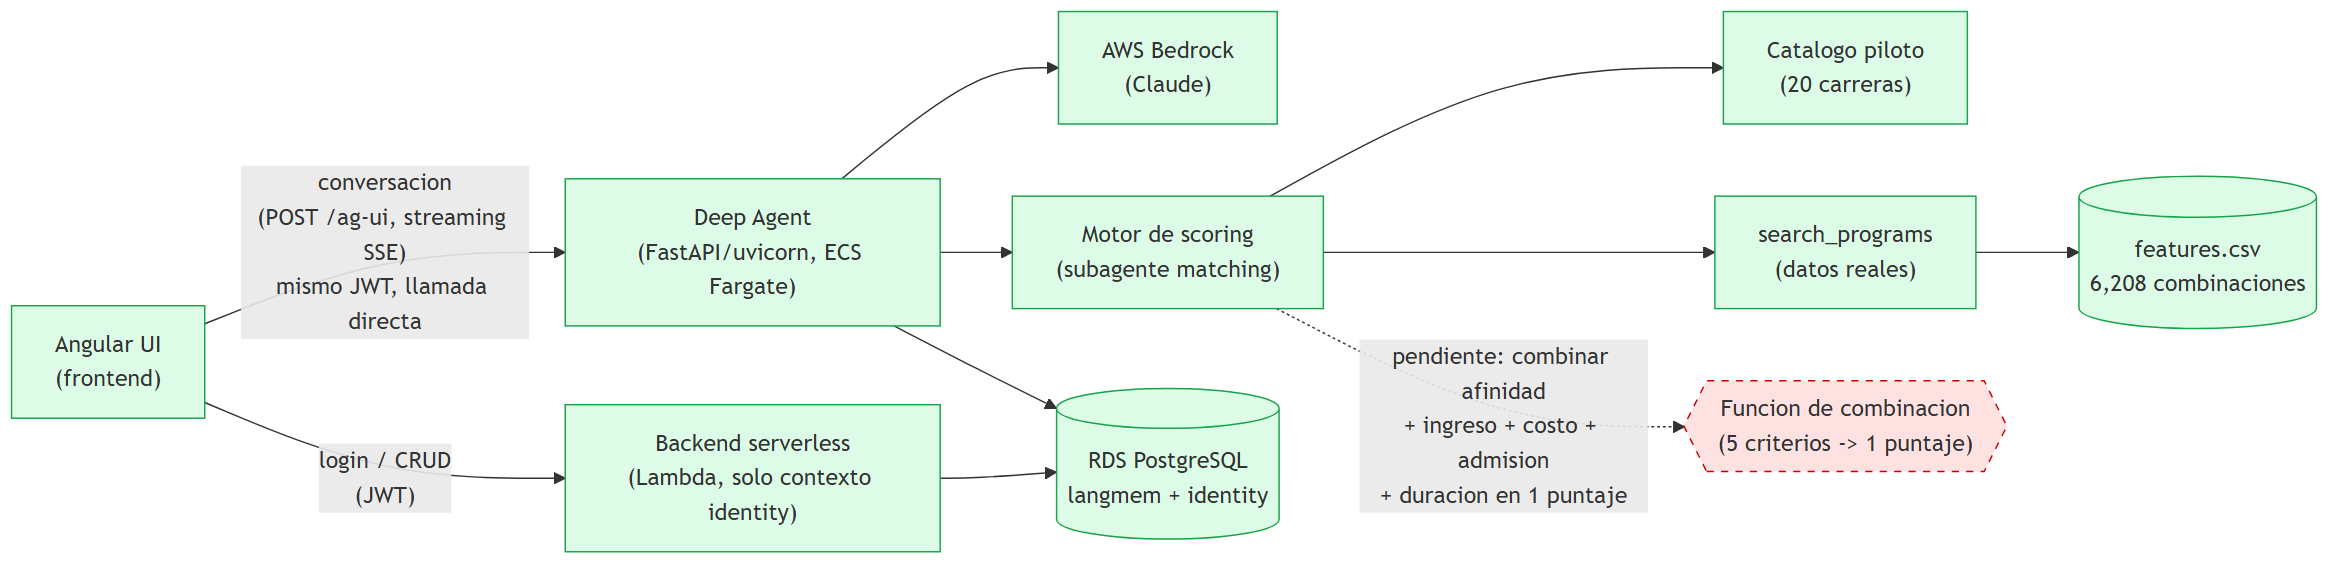
\includegraphics[width=0.95\linewidth]{fig-arquitectura-logica_v2.png}
    \caption{Arquitectura l\'ogica de componentes: el frontend se conecta
    \textbf{directamente} al backend (autenticaci\'on/CRUD) y al agente
    (conversaci\'on), sin proxy entre ambos.}
    \label{fig:architecture}
\end{figure}

\emph{Nota:} el frontend Angular llama a \textbf{ambos servicios de forma
directa} --- al backend serverless para autenticaci\'on y operaciones CRUD, y
al agente (\texttt{POST /ag-ui}, \emph{streaming} SSE) para la conversaci\'on
--- reutilizando el mismo JWT en ambas llamadas; \textbf{no hay} un
\emph{proxy} del backend hacia el agente, decisi\'on documentada
expl\'icitamente en el ADR-012 del backend. El agente corre detr\'as de su
propio \emph{Application Load Balancer} p\'ublico (no detr\'as de API
Gateway), precisamente porque el \emph{timeout} fijo de 30s de API Gateway
HTTP API cortar\'ia el \emph{streaming} SSE de \texttt{/ag-ui}. La
Figura~\ref{fig:architecture} representa el dise\~no objetivo de la
arquitectura a nivel de componentes l\'ogicos (no de despliegue): el agente ya
conecta tanto la afinidad RIASEC (cat\'alogo piloto) como los datos reales de
\texttt{features.csv} v\'ia \texttt{search\_programs}; lo que falta del nodo
marcado en rojo es el \textbf{motor de scoring} que combine ambos en un
puntaje ponderado \'unico (detalle m\'as abajo). La base de datos
relacional del proyecto es \textbf{Amazon RDS para PostgreSQL} (no Aurora); se
usa hoy para la persistencia de memoria del agente (ver subsecci\'on
siguiente) y para el dominio \texttt{identity} del backend.

\begin{landscape}
\begin{figure}[H]
    \centering
    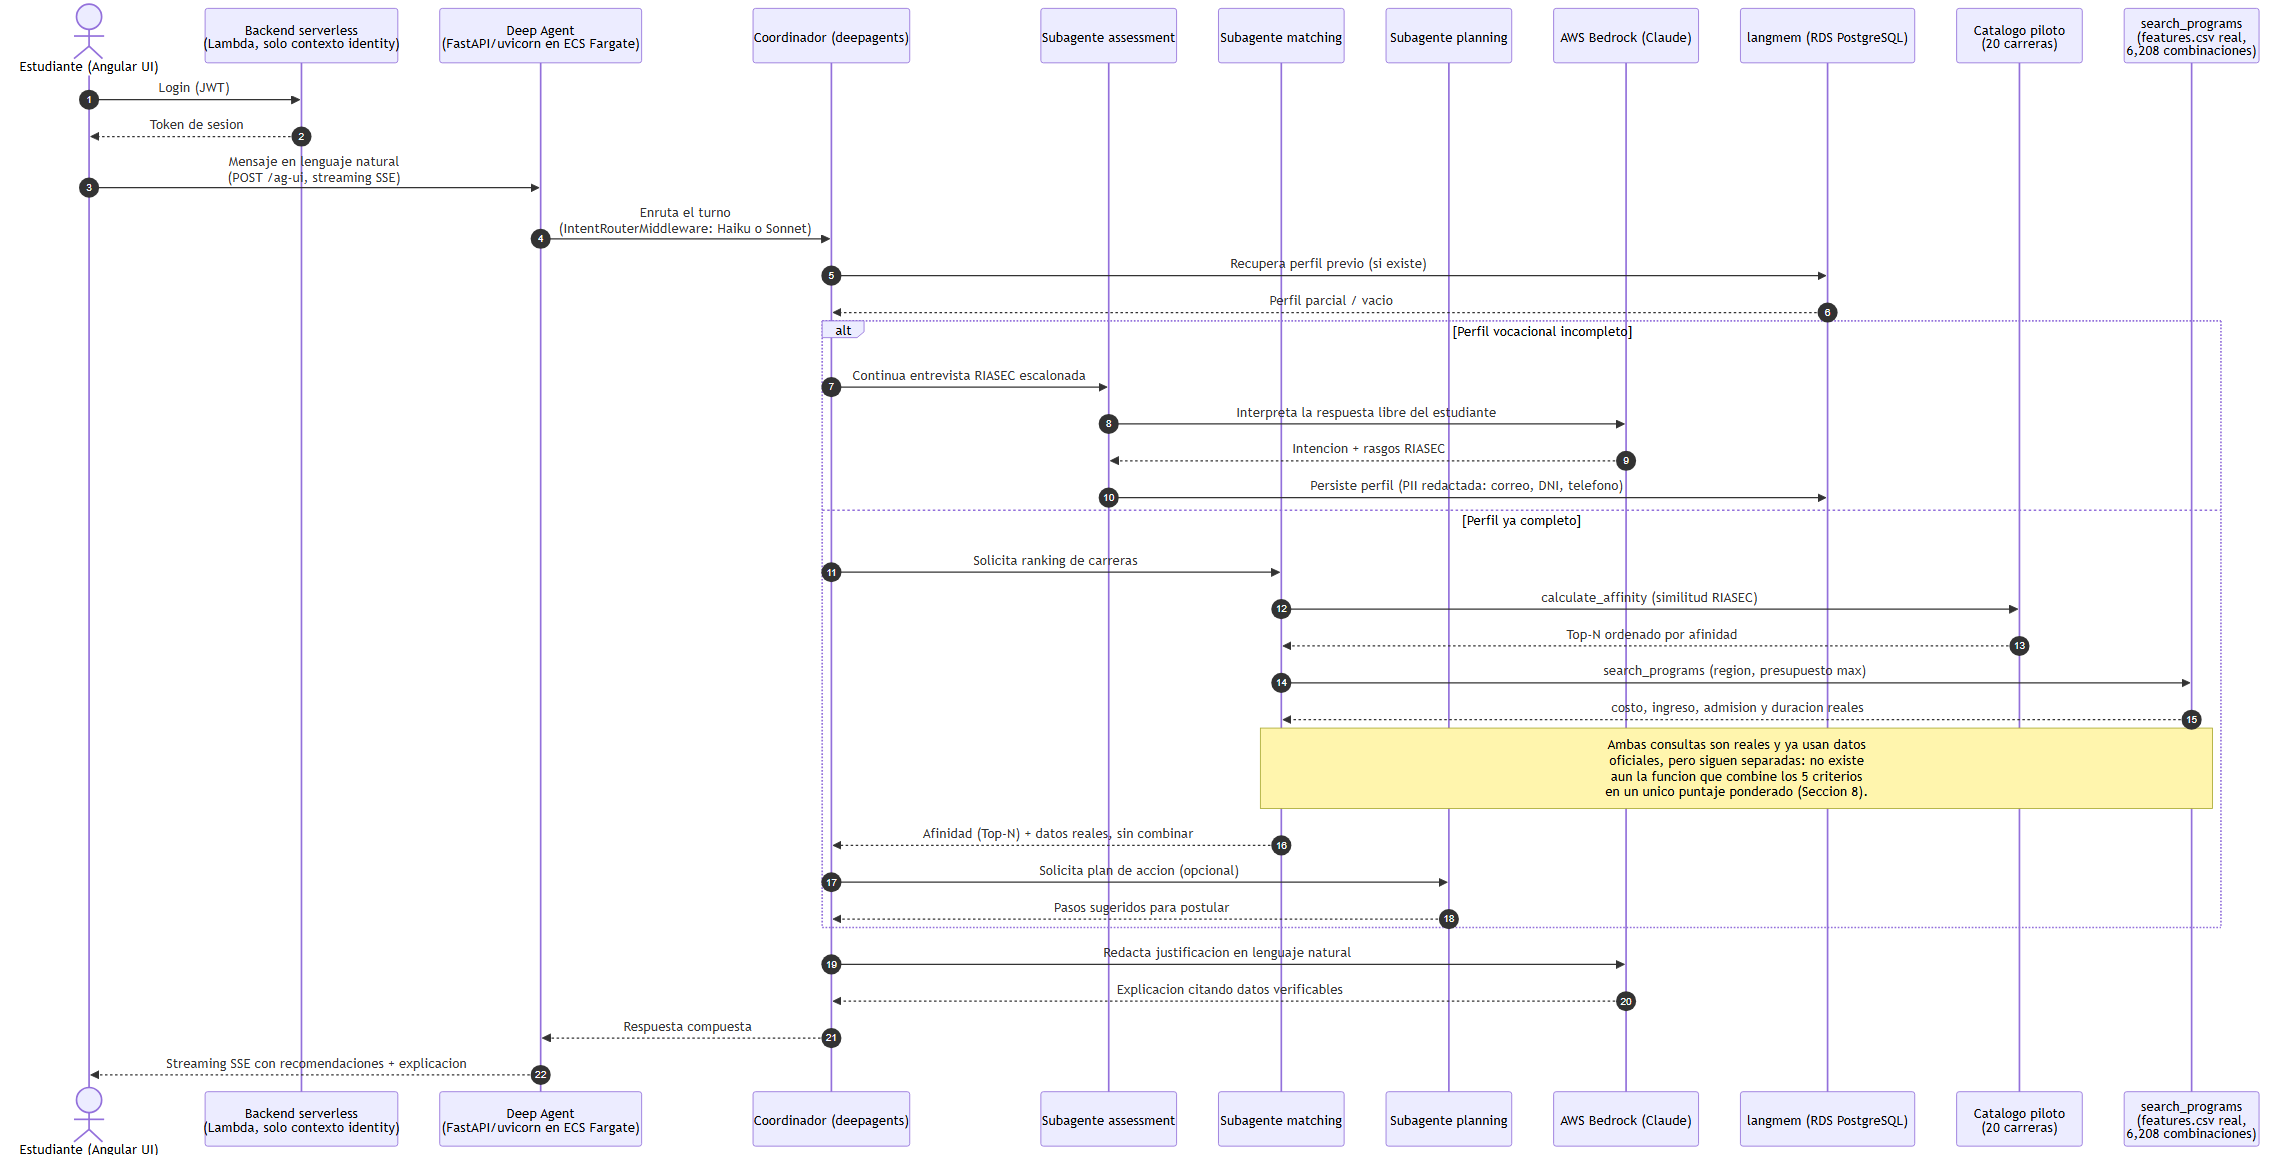
\includegraphics[width=0.92\linewidth]{fig-secuencia-conversacion_v2.png}
    \caption{Secuencia de una conversaci\'on t\'ipica, desde el mensaje del
    estudiante hasta la respuesta con recomendaciones explicadas.}
    \label{fig:conversation-sequence}
\end{figure}
\end{landscape}

\subsection{Agente conversacional (Deep Agent / deepagents)}

El agente se implementa en \textbf{Python} como un \emph{Deep Agent} construido
con el \emph{harness} \texttt{deepagents} ---del ecosistema
\emph{LangChain/LangGraph}--- que \textbf{coordina tres subagentes
especializados}: \texttt{assessment} (perfil vocacional RIASEC),
\texttt{matching} (afinidad, ranking de carreras y su aterrizaje en
universidades e institutos reales del Per\'u) y \texttt{planning} (plan de
acci\'on para la carrera elegida; ver Secci\'on~\ref{sec:prompts} para el
detalle de cada \emph{system prompt}).

\paragraph{Despliegue: contenedor en ECS Fargate, no AgentCore Runtime.} El
agente corri\'o inicialmente sobre AWS Bedrock AgentCore; la infraestructura
actual (m\'odulo \texttt{agent-service} de
\texttt{spark-match-02-infrastructure}) lo empaqueta en un \textbf{contenedor
Docker} y lo despliega en \textbf{AWS ECS Fargate} (ARM64) detr\'as de un
Application Load Balancer (raz\'on del cambio y detalle de despliegue en la
Secci\'on~\ref{sec:orchestration}).

\paragraph{Memoria del agente.} El perfil y las preferencias del estudiante se
persisten con \texttt{langmem} (\texttt{create\_manage\_memory\_tool} /
\texttt{create\_search\_memory\_tool}) bajo un espacio de nombres asociado al
usuario autenticado (JWT), respaldado por \textbf{RDS PostgreSQL} en producci\'on
(en memoria durante desarrollo/tests). En paralelo, un extractor de perfil en
segundo plano (\texttt{StudentProfile}) resume la conversaci\'on completa de
forma as\'incrona. Antes de persistir cualquier contenido, se redactan correos,
DNI y tel\'efonos peruanos (\emph{PII redaction}), de modo que la memoria de
largo plazo nunca almacena datos personales sensibles en texto plano.

El LLM (Claude en Bedrock) se resuelve a partir de la configuraci\'on de la
aplicaci\'on, que define dos modelos --- uno robusto para razonamiento y uno
r\'apido/econ\'omico para turnos simples, seleccionados por el enrutador de
intenci\'on descrito en la Secci\'on~\ref{sec:model-data} ---:

\begin{lstlisting}[style=pythonstyle, caption={Configuracion real de modelos (src/config/settings.py)}, label={lst:agent}]
model_id: str = "us.anthropic.claude-sonnet-4-5-20250929-v1:0"       # razonamiento
fast_model_id: str = "us.anthropic.claude-haiku-4-5-20251001-v1:0"   # turnos simples
\end{lstlisting}

\begin{figure}[H]
    \centering
    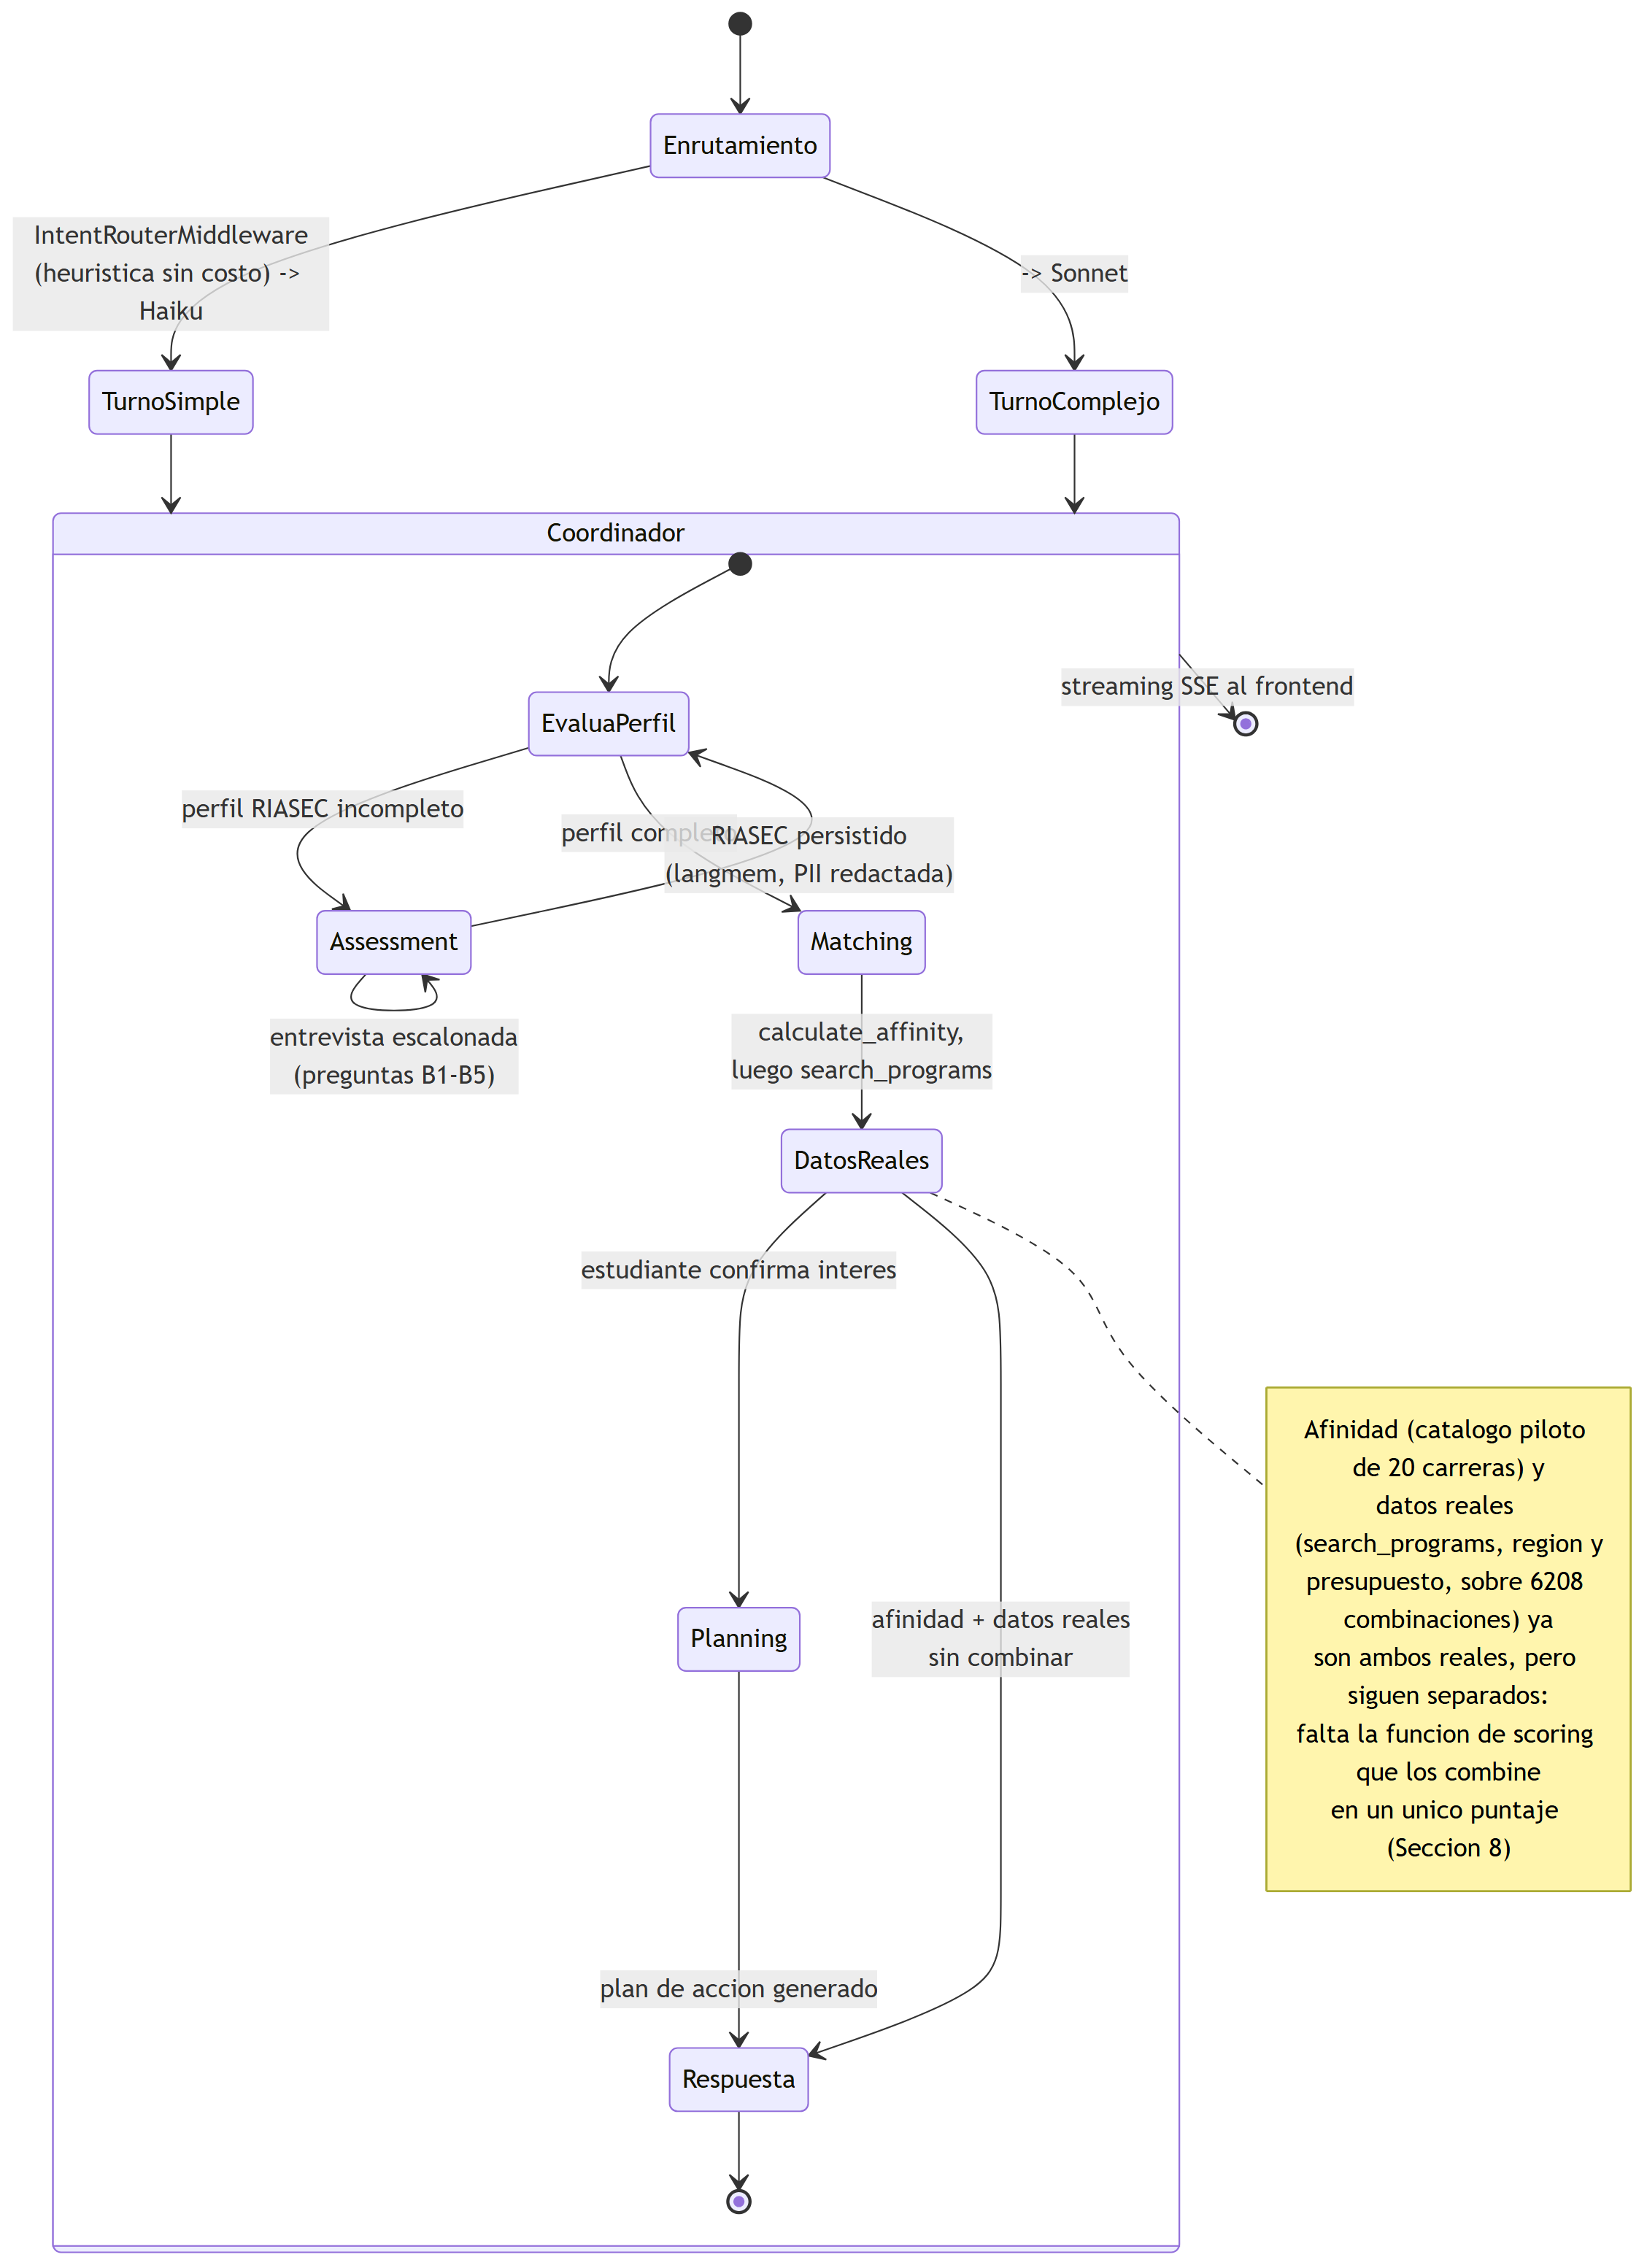
\includegraphics[width=\linewidth]{fig-estados-agente_v2.png}
    \caption{M\'aquina de estados del Deep Agent: enrutamiento por intenci\'on
    y coordinaci\'on de los tres subagentes especializados.}
    \label{fig:agent-states}
\end{figure}

\subsection{Motor de scoring (5 criterios)}

Cuando el agente entrega los pesos, el motor asigna un puntaje a cada
combinaci\'on carrera--universidad. La f\'ormula, con cinco criterios, es:

\[
\text{Score} = w_1\,\text{Afinidad} + w_2\,\text{Ingreso} + w_3\,\text{Costo}
             + w_4\,\text{Admisi\'on} + w_5\,\text{Duraci\'on}
\]

donde la \textbf{Afinidad} se calcula con el modelo \emph{RIASEC} de Holland
(compatibilidad entre el c\'odigo de 3 letras del estudiante y el de la carrera);
el \textbf{Ingreso} usa el sueldo promedio de egresados; el \textbf{Costo}
favorece las opciones m\'as accesibles; la \textbf{Admisi\'on} se basa en la tasa
de ingresantes/postulantes; y la \textbf{Duraci\'on} favorece carreras m\'as
cortas. Todas las variables vienen normalizadas en $[0,1]$ desde el pipeline. Los
pesos $w_1,\dots,w_5$ \textbf{no son fijos}: los infiere din\'amicamente el LLM en
cada sesi\'on, suman 1 y pueden ser 0 si el estudiante indica que un criterio no
le importa.

\begin{table}[H]
\centering
\begin{tabular}{@{}lcccccc@{}}
\toprule
\textbf{Carrera -- Universidad} & \textbf{Afin.} & \textbf{Ing.} & \textbf{Costo} & \textbf{Adm.} & \textbf{Dur.} & \textbf{Score} \\
\midrule
Estad\'istica -- UNMSM     & 95 & 85 & 90 & 60 & 80 & \textbf{86.0} \\
Econom\'ia -- UNMSM        & 80 & 82 & 88 & 55 & 80 & 79.2 \\
Ing.\ Industrial -- UNI    & 70 & 80 & 70 & 50 & 60 & 69.0 \\
\bottomrule
\end{tabular}
\caption{Ejemplo ilustrativo con pesos $(0.35, 0.25, 0.15, 0.10, 0.15)$. Los valores se muestran en escala 0--100 para facilitar la lectura; el pipeline trabaja en $[0,1]$.}
\label{tab:scoring-example}
\end{table}

Como ilustra la Tabla~\ref{tab:scoring-example}, el sistema ordena los resultados de mayor a menor y genera un ranking Top-N.
Luego el agente redacta la justificaci\'on, por ejemplo: \textit{``Te
recomendamos Estad\'istica en la UNMSM porque presenta una fuerte alineaci\'on
con tus intereses cuantitativos, tiene uno de los mejores ingresos promedio
dentro de las carreras anal\'iticas y mantiene costos relativamente bajos''.}

\paragraph{Estado de implementaci\'on.} La herramienta
\texttt{calculate\_affinity} del agente ya calcula el criterio de
\textbf{afinidad} (similitud RIASEC posicional) y ordena un Top-N por ese
criterio --- es, a la fecha, el \'unico de los cinco que el motor de
\emph{scoring} pondera dentro de un puntaje. Los otros cuatro criterios ---
\textbf{ingreso}, \textbf{costo}, \textbf{admisi\'on} y \textbf{duraci\'on} ---
ya est\'an calculados y normalizados por el \emph{pipeline} de datos
(Secci\'on~\ref{sec:model-data}), y desde la herramienta
\texttt{search\_programs} el agente puede consultarlos directamente sobre el
dataset completo de 6\,208 combinaciones carrera--instituci\'on, con cifras
reales de costo, ingreso, admisi\'on y duraci\'on en vez de datos gen\'ericos.
Lo que todav\'ia falta es la \textbf{funci\'on de combinaci\'on}: hoy el agente
presenta esos cuatro criterios junto a la afinidad para que el LLM razone
sobre ellos en su respuesta, pero no existe a\'un el c\'odigo que los combine
en un \'unico puntaje ponderado con los pesos $w_1,\dots,w_5$ de la
f\'ormula anterior; el ejemplo num\'erico de la Tabla~\ref{tab:scoring-example}
sigue siendo, por tanto, ilustrativo del dise\~no objetivo y no un resultado
medido. Ver Secci\'on~\ref{sec:results} para el detalle del alcance
implementado y el trabajo pendiente.

\subsection{Backend serverless}

El backend de plataforma (operaciones CRUD, gesti\'on de sesiones) sigue un
enfoque \emph{serverless} orientado a dominios (DDD): \textbf{TypeScript} sobre
AWS Lambda + EventBridge, empaquetado con AWS SAM. A la fecha implementa
\'unicamente el contexto \texttt{identity} (registro, login, roles,
desactivaci\'on de usuarios y auditor\'ia); el contexto de \emph{matching}/
recomendaci\'on todav\'ia no existe en esta capa (ver
Secci\'on~\ref{sec:results}). El backend cumple el rol de exposici\'on y
operaciones CRUD, sin l\'ogica de IA.

\subsection{Frontend}

El frontend es una SPA en \textbf{Angular 21} con Angular Material, organizada
por \emph{features} (\texttt{auth}, \texttt{chat}, \texttt{assessment},
\texttt{careers}, \texttt{filters}, \texttt{results}, \texttt{reports},
\texttt{profile} y \texttt{landing}). Cada feature tiene su propio
componente, servicio y pruebas unitarias; ya no es un simple \emph{scaffold}
vac\'io, aunque su integraci\'on end-to-end con el agente desplegado todav\'ia
est\'a en desarrollo.

Para acceder a la app es necesario crear una cuenta llenando el formulario de
registro con nombre completo, correo, contrase\~na, edad, regi\'on y \emph{área
de interés}. Luego se ingresa con el correo y la contrase\~na creados. En la
demo de prueba se puede usar el usuario \texttt{ftapara@unsa.edu.pe} con
contrase\~na \texttt{qwerty123}. El registro se realiza en
\url{https://d3sx4v4l1enpvk.cloudfront.net/auth/register}.

\begin{figure}[H]
    \centering
    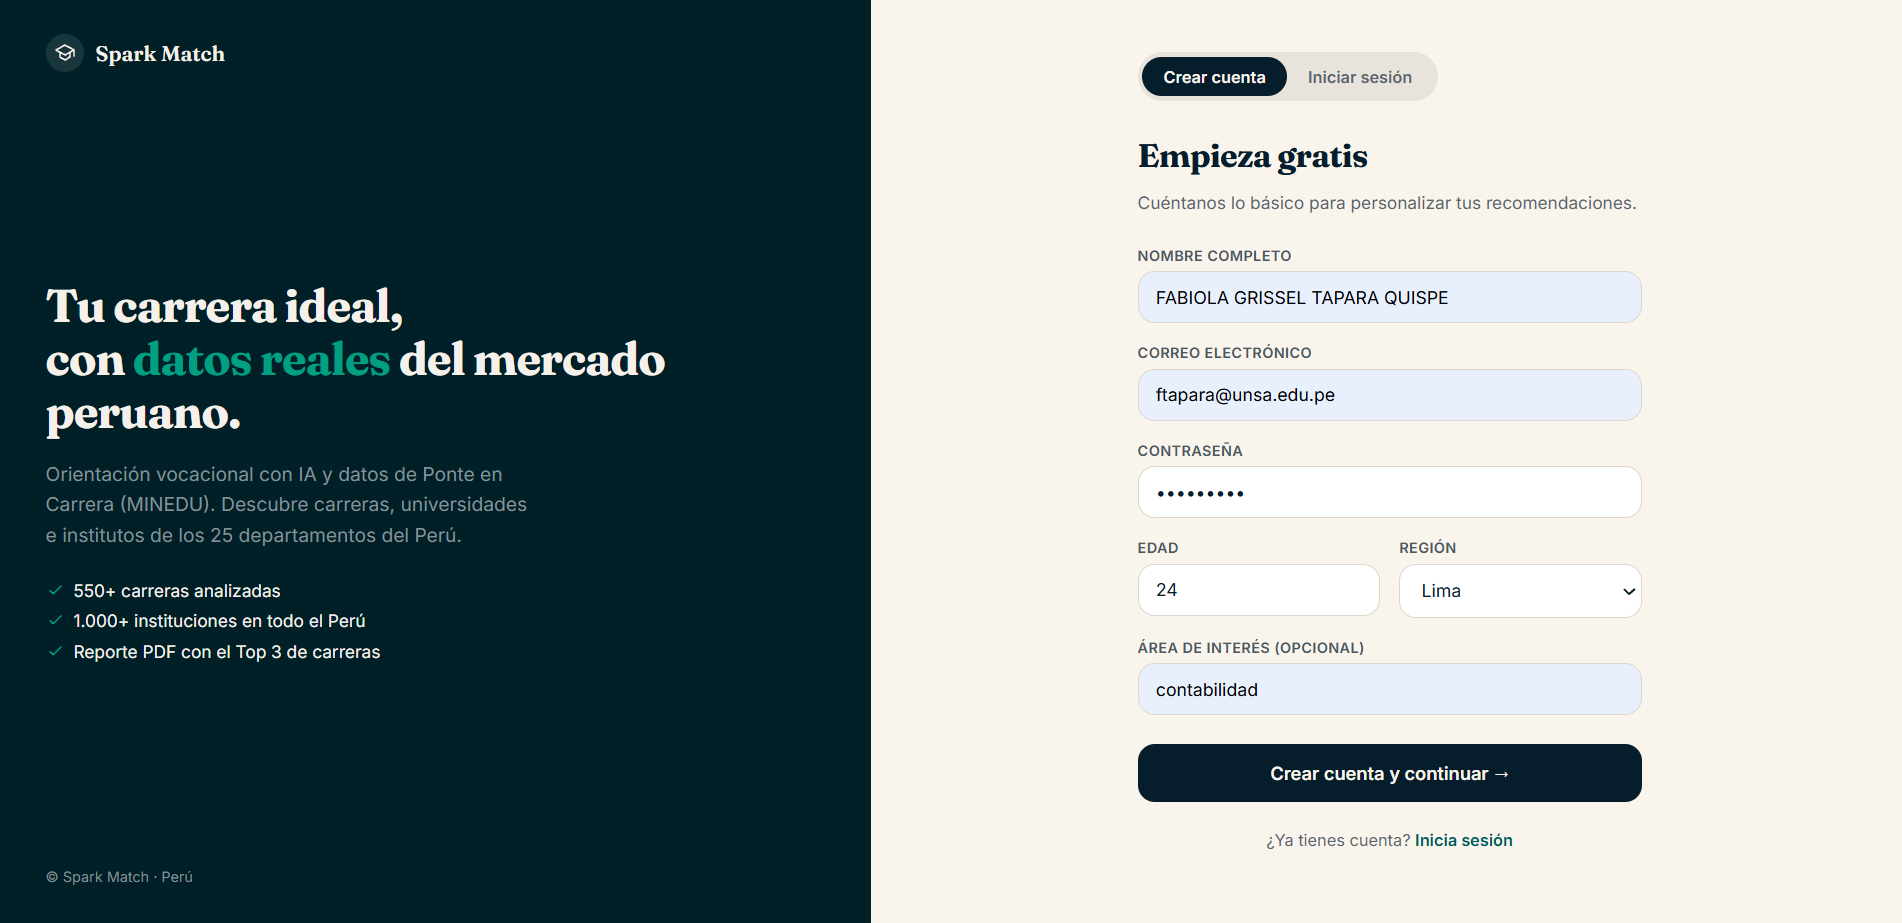
\includegraphics[width=0.95\linewidth]{crear cuenta.png}
    \caption{Formulario de registro del frontend de Spark Match.}
    \label{fig:fw-register}
\end{figure}

\begin{figure}[H]
    \centering
    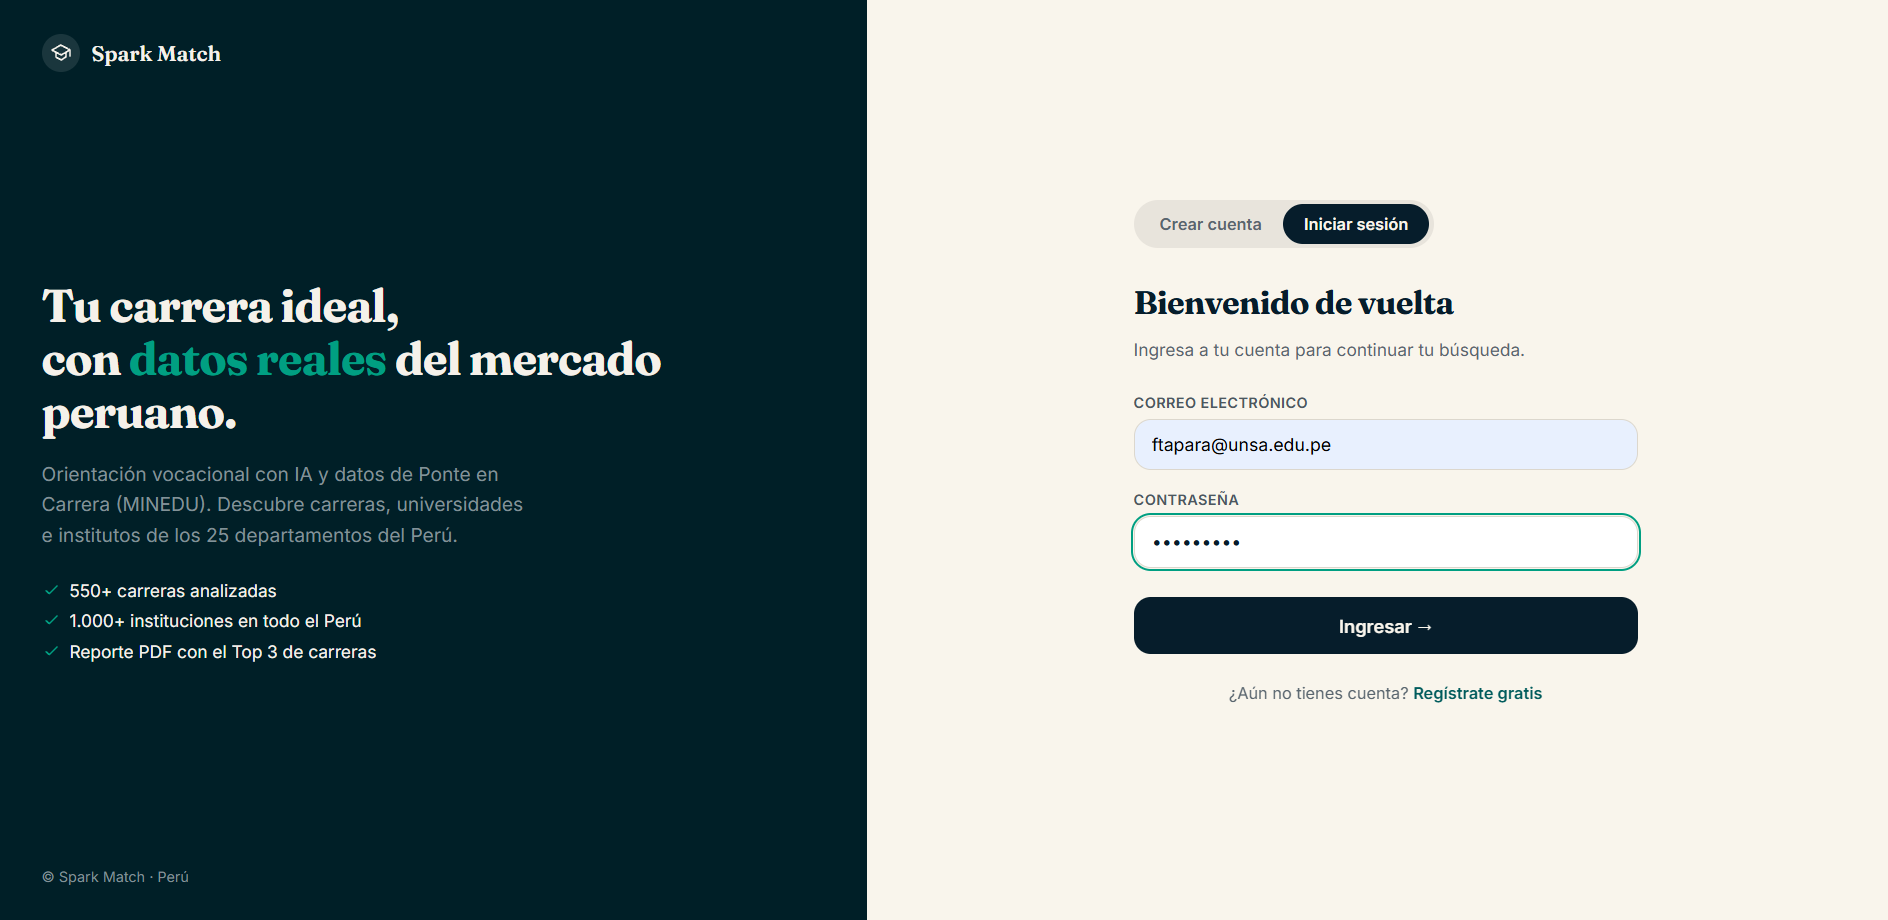
\includegraphics[width=0.95\linewidth]{iniciar sesion.png}
    \caption{Pantalla de inicio de sesi\'on del frontend.}
    \label{fig:fw-login}
\end{figure}

\begin{figure}[H]
    \centering
    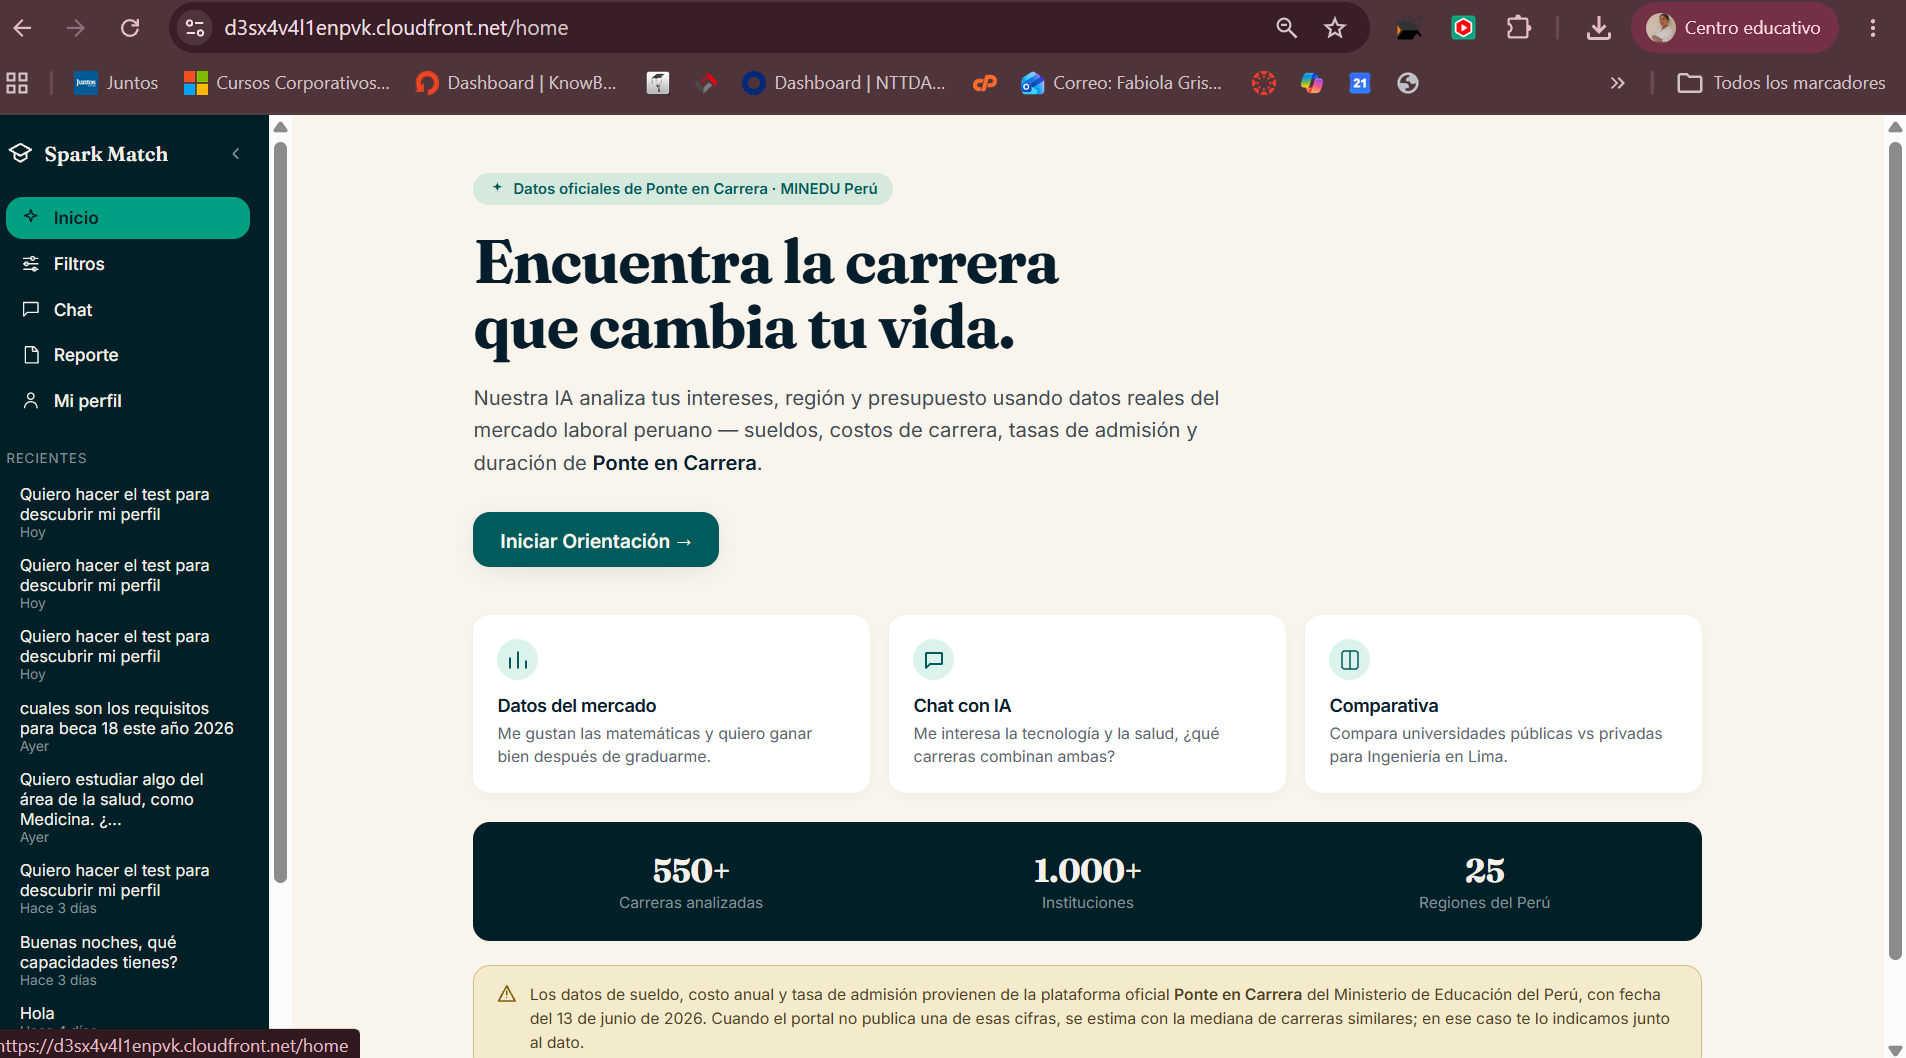
\includegraphics[width=0.95\linewidth]{inicio.png}
    \caption{Vista de inicio del usuario en la aplicaci\'on Spark Match.}
    \label{fig:fw-home}
\end{figure}

\begin{figure}[H]
    \centering
    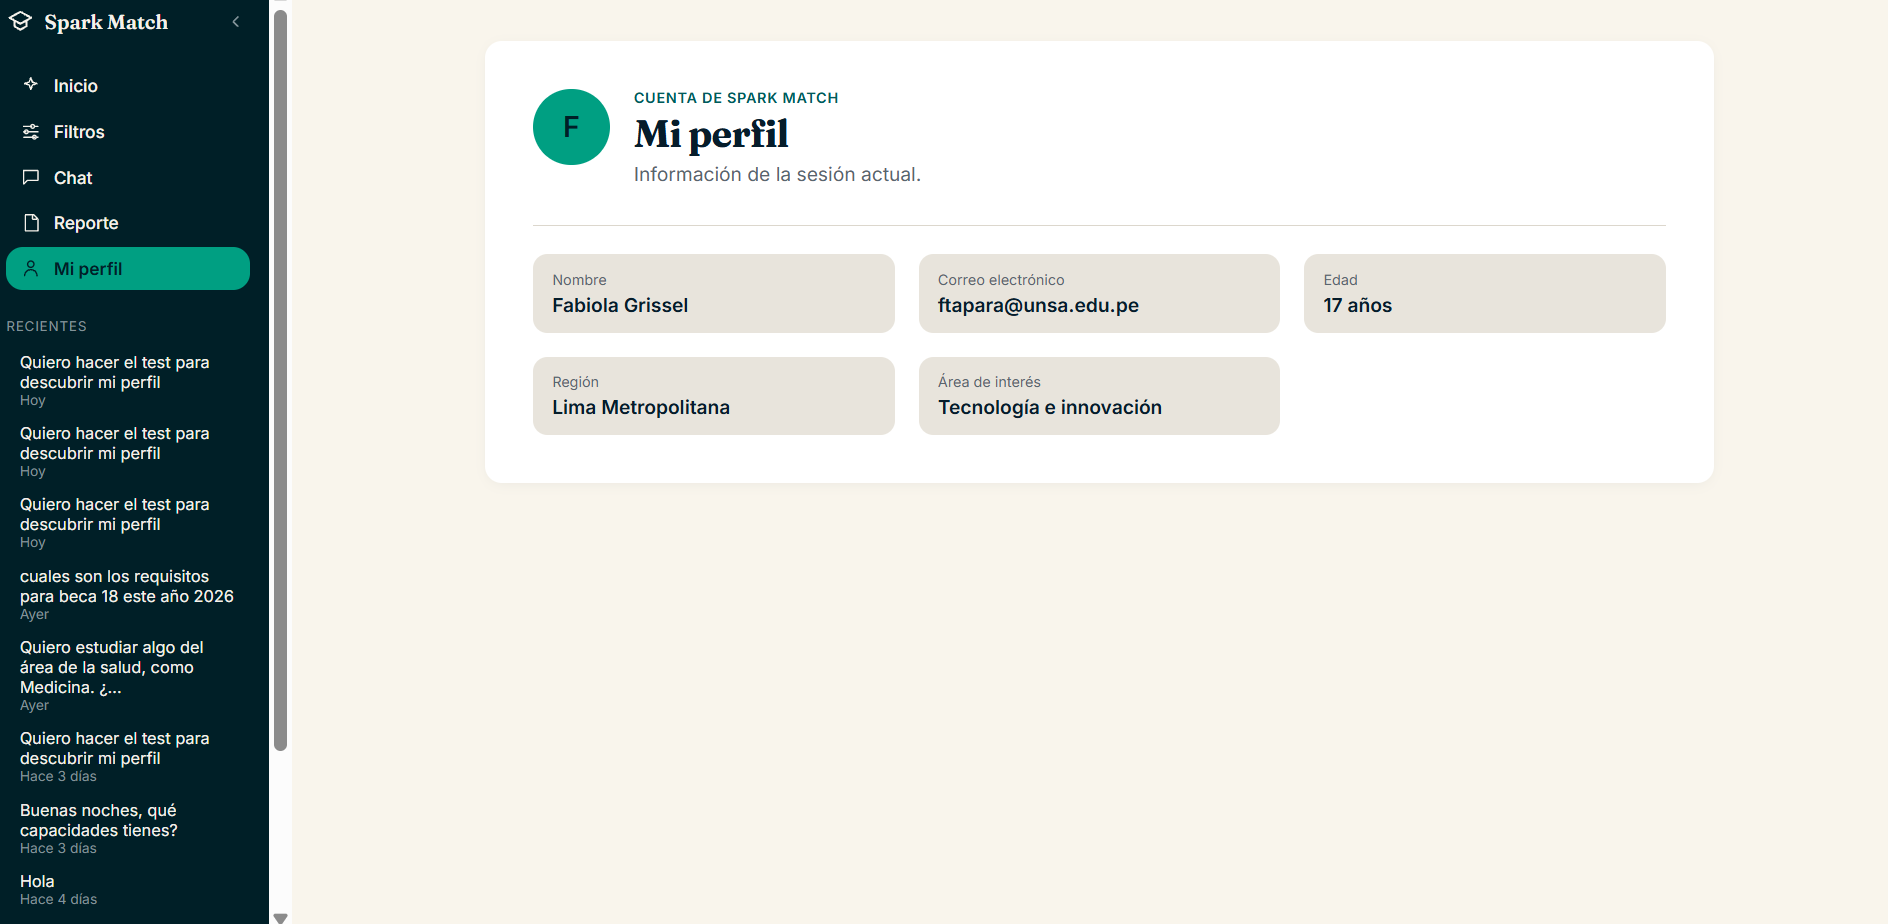
\includegraphics[width=0.95\linewidth]{perfil.png}
    \caption{Pantalla de perfil del estudiante, donde se muestran sus datos y preferencias.}
    \label{fig:fw-profile}
\end{figure}

\begin{figure}[H]
    \centering
    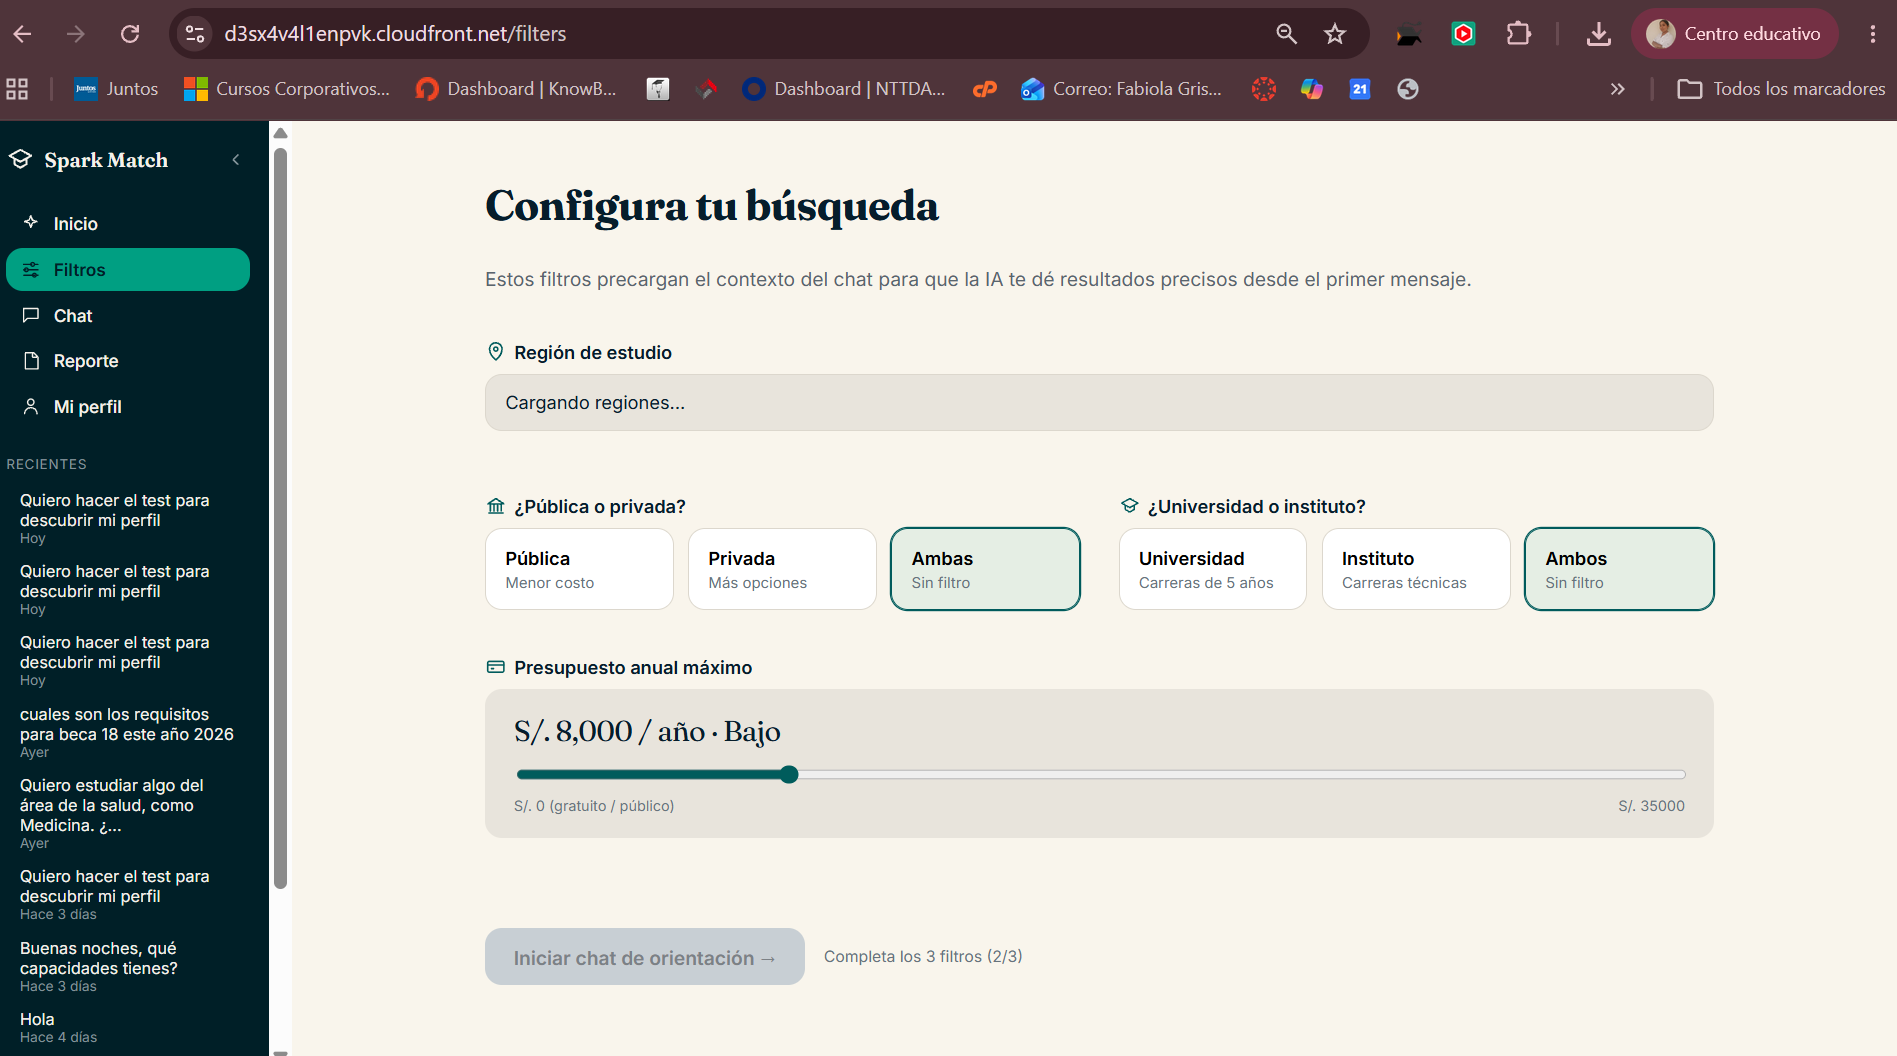
\includegraphics[width=0.95\linewidth]{filtros.png}
    \caption{Vista de filtros del frontend, que permite ajustar la orientaci\'on por regi\'on, tipo de instituci\'on y presupuesto.}
    \label{fig:fw-filters}
\end{figure}

La grabaci\'on del demo est\'a disponible en
\url{https://youtu.be/c_wMR6HVe1M} y muestra el flujo completo de registro,
inicio de sesi\'on, entrevista vocacional y recomendaciones explicadas.

El dise\~no privilegia la separaci\'on de responsabilidades (UI / API /
agente / scoring / datos), la configuraci\'on por variables de entorno y una
API sin estado (las sesiones se persisten en base de datos, no en memoria).

\paragraph{Lenguaje del n\'ucleo.} El \textbf{n\'ucleo de IA/ML del proyecto est\'a
implementado en Python}: el agente conversacional (\texttt{deepagents}), el motor
de scoring (Pandas/NumPy), el \emph{pipeline} de datos y el framework de
evaluaci\'on.

% ============================================================================
% Seccion 5: Orquestacion y Despliegue
% TFP - Rubrica: 2 puntos
% ============================================================================
\section{Orquestaci\'on y despliegue}

% TODO: Documentar el Dockerfile del backend, docker-compose para desarrollo
% local, manifest de Kubernetes (o ECS Fargate) para produccion, y los
% GitHub Actions workflows (build, test, deploy).

\subsection{API REST con FastAPI}

[Detallar la implementacion de FastAPI:
- Estructura del proyecto: routers, services, repositories, models.
- Validacion con Pydantic v2.
- Documentacion automatica OpenAPI en \texttt{/docs}.
- Middlewares: CORS, logging, rate limiting, autenticacion (si aplica).
- Tests: pytest + httpx.AsyncClient con coverage $\geq$ 80\%.]

\begin{lstlisting}[style=bashstyle, caption={Ejecucion local de la API}, label={lst:run-api}]
uvicorn spark_match.main:app --reload --host 0.0.0.0 --port 8000
# Swagger UI: http://localhost:8000/docs
\end{lstlisting}

\subsection{Contenerizaci\'on con Docker}

[Describir el Dockerfile:
- Imagen base: \texttt{python:3.12-slim}.
- Multi-stage build para reducir tamano final.
- Usuario no-root para seguridad.
- Capa de dependencias separada del codigo (cache de capas).
- Healthcheck definido.
- Variables de entorno via \texttt{env\_file}.]

\begin{lstlisting}[style=yamlstyle, caption={docker-compose.yml para desarrollo local}, label={lst:compose}]
version: "3.9"
services:
  api:
    build: ./spark-match-03-backend
    ports: ["8000:8000"]
    env_file: .env
    depends_on: [postgres, chromadb]
  frontend:
    build: ./spark-match-04-frontend
    ports: ["4200:4200"]
  postgres:
    image: postgres:16-alpine
    environment:
      POSTGRES_DB: sparkmatch
      POSTGRES_PASSWORD: dev
    volumes: ["pgdata:/var/lib/postgresql/data"]
volumes:
  pgdata:
\end{lstlisting}

\subsection{Infraestructura como c\'odigo (Terraform)}

[Detcribir los recursos provisionados en AWS:
- VPC con subnets publicas/privadas.
- ECS Fargate (o EKS) para el backend.
- RDS PostgreSQL (multi-AZ).
- S3 para datasets versionados (DVC remote).
- CloudFront + S3 para el frontend Angular.
- Secrets Manager para API keys.
- IAM roles con least privilege.]

\begin{lstlisting}[style=yamlstyle, caption={Modulo Terraform: ECS Fargate service}, label={lst:tf-ecs}]
resource "aws_ecs_service" "spark_match_api" {
  name            = "spark-match-api"
  cluster         = aws_ecs_cluster.main.id
  task_definition = aws_ecs_task_definition.api.arn
  desired_count   = 2
  launch_type     = "FARGATE"

  network_configuration {
    subnets         = aws_subnet.private[*].id
    security_groups = [aws_security_group.api.id]
  }

  load_balancer {
    target_group_arn = aws_lb_target_group.api.arn
    container_name   = "api"
    container_port   = 8000
  }
}
\end{lstlisting}

\subsection{CI/CD con GitHub Actions}

[Detallar los workflows:
- \texttt{ci.yml} (reusable): lint + tests + build de imagen Docker.
- \texttt{deploy-staging.yml}: push a staging tras merge a \texttt{main}.
- \texttt{deploy-prod.yml}: despliegue a produccion con aprobacion manual.
- Versionado semantico automatico con release-please.
- Escaneo de vulnerabilidades: Trivy + Snyk.]

\begin{lstlisting}[style=yamlstyle, caption={Workflow reutilizable de CI}, label={lst:gh-actions}]
name: CI
on:
  workflow_call:
jobs:
  test:
    runs-on: ubuntu-latest
    steps:
      - uses: actions/checkout@v6
      - uses: actions/setup-python@v6
        with: {python-version: "3.12"}
      - run: pip install -r requirements.txt
      - run: pytest --cov=app --cov-fail-under=80
  docker:
    needs: test
    runs-on: ubuntu-latest
    steps:
      - uses: actions/checkout@v6
      - run: docker build -t $IMAGE:${{ github.sha }} .
      - run: docker push $IMAGE:${{ github.sha }}
\end{lstlisting}

\subsection{Despliegue en la nube (AWS)}

[Resumen del entorno productivo:
- Region: us-east-1 (o sa-east-1 para menor latencia en Per'u).
- Cluster: ECS Fargate con auto-scaling (CPU 70\%).
- Base de datos: RDS PostgreSQL 16.
- CDN: CloudFront.
- Costos estimados: USD/mes [definir tras el despliegue].
- URL de demo: \url{https://spark-match.app} [placeholder].]
% ============================================================================
% Seccion 6: Monitoreo y Mantenimiento
% TFP - Rubrica: 2 puntos
% ============================================================================
\section{Monitoreo y mantenimiento}

% TODO: Documentar las herramientas de monitoreo elegidas, las metricas
% capturadas (latencia, throughput, tasa de exito, uso de tokens, costos
% LLM), la gestion de drift en el dataset y los mecanismos de alerta.

\subsection{Estrategia de monitoreo}

[Describir el stack de observabilidad:
- \textbf{MLflow Tracking}: experimentos, parametros, metricas, artefactos del motor de scoring.
- \textbf{LangSmith} o \textbf{Bedrock Agents tracing}: trazas de invocaciones del LLM (latencia, tokens, costo por llamada).
- \textbf{Prometheus}: metricas de aplicacion (request rate, error rate, latency).
- \textbf{Grafana}: dashboards operativos.
- \textbf{CloudWatch}: logs y metricas de infraestructura AWS.
- \textbf{Sentry}: captura de excepciones en frontend y backend.]

\begin{lstlisting}[style=pythonstyle, caption={Tracking de un experimento de motor de scoring con MLflow}, label={lst:mlflow}]
import mlflow

mlflow.set_tracking_uri("https://mlflow.spark-match.app")
mlflow.set_experiment("scoring-engine")

with mlflow.start_run(run_name="weighted-v3"):
    mlflow.log_param("weights", {"salario": 0.4, "costo": 0.3, ...})
    mlflow.log_metric("ndcg@5", 0.82)
    mlflow.log_metric("mae_salary", 312.5)
    mlflow.sklearn.log_model(model, "model")
\end{lstlisting}

\subsection{M\'etricas de desempe\~no en producci\'on}

[Tabla de SLIs/SLOs:
- Latencia p50/p95/p99 del endpoint \texttt{/chat} (<2s / <5s / <10s).
- Throughput: requests/minuto.
- Tasa de exito (HTTP 2xx) > 99\%.
- Tokens consumidos por conversacion (mediana).
- Costo LLM por conversacion (USD).
- Satisfaccion del usuario (thumbs up/down post-respuesta).
- Precision del Top-N vs decision final del usuario (medido por feedback).]

\subsection{Gesti\'on de drift}

[Politica de monitoreo de drift:
- \textbf{Drift de datos}: comparacion semanal de la distribucion de features (KS test, PSI) entre el dataset actual y el de entrenamiento.
- \textbf{Drift de modelo}: degradacion sostenida del feedback positivo (umbral: <70\% durante 7 dias).
- \textbf{Drift de concepto}: cambios en la oferta educativa (nuevas carreras, universidades cerradas) detectados por DVC diff.
- Reentrenamiento: pipeline automatizado en GitHub Actions al detectar drift $>$ umbral.]

\subsection{Logging y alertas}

[Configuracion de logging y alertas:
- Logs estructurados JSON (nivel INFO/WARN/ERROR).
- Correlacion con \texttt{trace\_id} propagado desde el frontend.
- Alertas en CloudWatch + Slack webhook:
  - Latencia p95 > 5s durante 5 min.
  - Error rate > 5\% durante 5 min.
  - Costo LLM diario > USD 50.
  - Drift detectado por el job semanal.]

\subsection{Plan de mantenimiento}

[Calendario de mantenimiento:
- Parches de seguridad: semanal (Dependabot + auto-merge de patches).
- Reentrenamiento del motor de scoring: mensual o por drift.
- Actualizacion del dataset: cada semestre (alineado con calendario academico).
- Rotacion de secretos: trimestral.
- Disaster recovery: backup diario de RDS + replicacion cross-region.]
% ============================================================================
% Seccion 7: Evaluacion de la Aplicacion
% TFP - Rubrica: 2 puntos
% ============================================================================
\section{Evaluaci\'on de la aplicaci\'on}

La evaluaci\'on combina indicadores t\'ecnicos y de negocio. Dado que en esta
etapa el sistema es un prototipo, se describe el \emph{marco de evaluaci\'on}
definido; los valores medidos se completar\'an con las pruebas finales.

\subsection{M\'etricas empleadas}

\paragraph{Recuperaci\'on y ranking.} Para el motor de scoring (ranking Top-N) se
emplean m\'etricas como \textbf{Recall@K} y relevancia frente a un conjunto de
casos de referencia, evaluando si las carreras pertinentes aparecen en el Top-N.

\paragraph{Extractor de preferencias (LLM).} Se mide la correcci\'on de los
campos estructurados (regi\'on, presupuesto, pesos, c\'odigo RIASEC) y la tasa de
JSON malformado.

\paragraph{Justificaci\'on en lenguaje natural (LLM).} Se usa un componente de
\textbf{LLM-as-judge} que puntu\'a las explicaciones del agente, complementado con
evaluaci\'on humana de claridad, relevancia y \emph{factualidad} (que la
explicaci\'on se sustente en los datos del ranking y no invente cifras).

\paragraph{Negocio.} Satisfacci\'on del usuario, pertinencia percibida de la
recomendaci\'on y, a futuro, tasa de aceptaci\'on de la carrera sugerida.

\subsection{Costos como KPI}

Se consideran KPI de costo el costo mensual de infraestructura (con \emph{AWS
Budgets} como control) y el consumo de tokens del LLM (observado v\'ia LangSmith).
Estos indicadores son relevantes por tratarse de un proyecto acad\'emico con
presupuesto acotado.

\subsection{Casos de prueba y validaci\'on}

La evaluaci\'on se apoya en un dataset de casos representativos que cubren
distintos perfiles de estudiante (por regi\'on, presupuesto y prioridades), sobre
los cuales se ejecuta el flujo completo (extracci\'on de preferencias
$\rightarrow$ scoring $\rightarrow$ justificaci\'on) y se contrastan las salidas
con lo esperado. Se contemplan del orden de \textbf{5--6 casos can\'onicos} (por
ejemplo, el estudiante de Cusco con presupuesto acotado de la Secci\'on~8).

\paragraph{Reto de los \emph{evals} en un sistema conversacional.} A diferencia de
una interacci\'on simple de pregunta--respuesta, aqu\'i la conversaci\'on es
\textbf{multi-turno}: para que un \emph{eval} sea representativo debe simular
varios mensajes del estudiante (saludo, aporte de preferencias, aclaraciones),
no un \'unico JSON de entrada. Por ello los casos de prueba se construyen como
\emph{guiones de conversaci\'on} y se eval\'uan con el \emph{LLM-as-judge}. Este
componente se implementa del lado de AWS y queda \textbf{pendiente} hasta que el
agente est\'e desplegado.

\subsection{Comparaci\'on de enfoques (resultados)}

Se compar\'o el enfoque propuesto (pesos din\'amicos inferidos por el LLM) frente a
dos \emph{baselines}, midiendo cu\'antas carreras del Top-5 comparte cada uno con el
enfoque propuesto para el caso de Cusco (288 candidatas tras los filtros):

\begin{table}[H]
\centering
\begin{tabular}{@{}lcl@{}}
\toprule
Enfoque & Top-5 en com\'un & Interpretaci\'on \\
\midrule
Pesos din\'amicos (propuesto) & --- & referencia \\
Pesos iguales (baseline 1)    & 1/5 & el ranking cambia casi por completo \\
Solo ingreso (baseline 2)     & 3/5 & los pesos s\'i modifican el resultado \\
\bottomrule
\end{tabular}
\caption{El motor de 5 factores no equivale a un \emph{baseline} simple.}
\label{tab:comparacion-enfoques}
\end{table}

\paragraph{Prueba de consistencia.} Para dos perfiles en Lima, uno que prioriza el
costo y otro el ingreso, el \'indice de accesibilidad de costo (\texttt{cost\_norm},
mayor $=$ m\'as accesible) del Top-10 fue \textbf{0.941} vs.\ \textbf{0.502}: el
motor entrega opciones m\'as accesibles a quien prioriza el costo, confirmando que
el ranking responde a las preferencias del estudiante.

\paragraph{Nota metodol\'ogica.} Estos resultados eval\'uan el \emph{motor de
recomendaci\'on} (determin\'istico) sobre \texttt{features.csv}; la evaluaci\'on de
las respuestas en lenguaje natural del agente (\emph{LLM-as-judge},
\emph{groundedness}) se realiza sobre el sistema desplegado.

\subsection{Limitaciones detectadas}

\begin{itemize}[noitemsep]
  \item Los datos de salario reflejan solo el empleo formal y pueden subestimar
        ingresos reales en ciertos rubros.
  \item Las carreras o universidades con pocos egresados producen promedios poco
        confiables.
  \item Los pesos y la f\'ormula de scoring de esta etapa son ilustrativos y
        requieren calibraci\'on con usuarios reales.
  \item El LLM puede generar pesos incoherentes ante mensajes ambiguos; por ello
        la explicaci\'on se ancla siempre en datos verificables del ranking.
  \item La evaluaci\'on humana est\'a limitada a un n\'umero reducido de usuarios
        de prueba en esta fase.
  \item La variable de \textbf{costo anual} es la menos confiable del dataset:
        aproximadamente el \textbf{50\%} de los registros est\'a vac\'io o imputado
        (19\% nulos, 31\% en cero, 50\% imputado). El motor usa la versi\'on
        normalizada e imputada (\texttt{cost\_norm}), por lo que el \emph{ranking}
        se mantiene v\'alido, pero los montos absolutos de costo no deben
        interpretarse de forma literal.
\end{itemize}

% ============================================================================
% Seccion 8: Resultados y Demostracion
% TFP - Rubrica: 2 puntos
% ============================================================================
\section{Resultados y demostraci\'on}
\label{sec:results}

\subsection{Estado del prototipo}

El c\'odigo del proyecto se organiza en la organizaci\'on de GitHub
\texttt{spark-match}, con repositorios separados por dominio (datos, backend,
agente, frontend, infraestructura, DevOps y art\'iculo). A la fecha est\'an
implementados:

\begin{itemize}[noitemsep]
  \item el \emph{pipeline de datos} que produce \texttt{features.csv} (6\,208
        combinaciones carrera--instituci\'on, 554 carreras \'unicas), con las
        variables de ingreso, costo, admisi\'on y duraci\'on ya normalizadas;
  \item el \emph{etiquetado RIASEC} de las carreras mediante el LLM en Bedrock;
  \item el \emph{agente conversacional} (Deep Agent) con cuatro herramientas
        operativas: evaluaci\'on de perfil RIASEC (\texttt{evaluate\_riasec\_}
        \texttt{profile}), b\'usqueda de carreras (\texttt{search\_careers}),
        c\'alculo de afinidad vocacional (\texttt{calculate\_affinity}) y
        b\'usqueda web de respaldo (\texttt{web\_search}), trazadas con
        LangSmith y con un framework de evaluaci\'on;
  \item los \emph{scaffolds} del backend serverless (TypeScript, contexto
        \texttt{identity}: autenticaci\'on, usuarios y auditor\'ia) y del
        frontend (Angular 21);
  \item la \emph{infraestructura} en Terraform con ambientes \texttt{dev} y
        \texttt{prod}.
\end{itemize}

\paragraph{Alcance real del motor de scoring (importante).} De los cinco
criterios dise\~nados (afinidad, ingreso, costo, admisi\'on, duraci\'on), a la
fecha \textbf{solo la afinidad vocacional (RIASEC) est\'a integrada} en la
herramienta \texttt{calculate\_affinity} del agente, y \'esta opera sobre un
\textbf{cat\'alogo piloto de 19 carreras} definidas manualmente en
\texttt{data/careers/} (con nombre, campo y perfil RIASEC, sin universidad,
ingreso, costo ni admisi\'on) --- \textbf{no} sobre las 6\,208 combinaciones de
\texttt{features.csv}. El backend serverless, por su parte, solo implementa el
contexto \texttt{identity}; no existe a\'un un contexto de \emph{matching} ni
una carga de \texttt{features.csv} en RDS PostgreSQL. En consecuencia, el
ranking multicriterio y el ejemplo num\'erico de la
Secci\'on~\ref{sec:implementation} describen el dise\~no objetivo del sistema,
no un resultado ya medido end-to-end. El trabajo pendiente para cerrar esta
brecha --- integrar ingreso, costo, admisi\'on y duraci\'on al agente, y
conectar su cat\'alogo con el dataset completo --- se detalla en
\texttt{DOCS/issues/issues-v1/}.

\subsection{Ejemplo de salida (caso can\'onico)}

\textbf{Caso:} estudiante de Cusco, presupuesto m\'aximo S/600/mes, prioridad en
salario y cercan\'ia geogr\'afica.

\textbf{Mensaje del usuario:} \textit{``Vivo en Cusco y mi presupuesto m\'aximo es
600 soles al mes. Me interesa algo con buenos sueldos pero tambi\'en quiero
quedarme cerca de casa''.}

\textbf{Preferencias extra\'idas por el LLM:}
\begin{lstlisting}[style=jsonstyle, caption={JSON de preferencias extraidas}, label={lst:json-prefs}]
{
  "region": "Cusco",
  "presupuesto_max": 600,
  "peso_afinidad": 0.15,
  "peso_ingreso": 0.45,
  "peso_costo": 0.30,
  "peso_admision": 0.05,
  "peso_duracion": 0.05
}
\end{lstlisting}

El motor de scoring aplica los filtros duros (regi\'on Cusco, presupuesto) y
ordena las combinaciones carrera--universidad por su puntaje, generando un ranking
Top-N. Finalmente, el agente redacta una justificaci\'on en lenguaje natural que
cita los datos que sustentan cada recomendaci\'on (ingreso promedio, costo,
afinidad).

\begin{figure}[H]
    \centering
    % \includegraphics[width=0.95\linewidth]{chat-screenshot.png}
    \caption{Captura de la interfaz conversacional de Spark Match (por incluir).}
    \label{fig:chat}
\end{figure}
% TODO (equipo): reemplazar por capturas reales de la app corriendo, el ranking
% Top-N de un caso real y el enlace a la demo/video.

\subsection{Evidencia funcional}

La demostraci\'on final mostrar\'a el flujo de extremo a extremo: el estudiante
conversa con el orientador, el agente construye su perfil y prioridades, el motor
de scoring genera el ranking Top-N sobre datos reales y el agente entrega las
recomendaciones explicadas. La evidencia incluir\'a:

\begin{itemize}[noitemsep]
  \item \textbf{Repositorios:} \url{https://github.com/spark-match}.
  \item \textbf{Demo / video:} enlace por definir tras el despliegue.
  \item \textbf{Capturas:} conversaci\'on real con el agente (Figura~\ref{fig:chat}),
        ranking Top-N y trazas de observabilidad en LangSmith.
\end{itemize}

% ============================================================================
% Seccion 9: Conclusiones
% TFP - Rubrica: 1 punto
% ============================================================================
\section{Conclusiones}

% TODO: Redactar 1-2 parrafos reflexivos sobre los logros principales,
% dificultades encontradas durante el desarrollo y principales aprendizajes.
% Cerrar con la evaluacion del impacto del proyecto.

\subsection{Logros principales}

[Resumen ejecutivo de lo que se logro:
- Sistema Spark Match desplegado end-to-end (Angular + FastAPI + LangChain + AWS).
- Pipeline de datos versionado con DVC y motor de scoring reproducible con MLflow.
- Agente conversacional capaz de interpretar preferencias libres y devolver rankings explicables.
- Evaluacion cuantitativa que muestra que el enfoque hibrido (LLM + scoring) supera a las baselines en NDCG@5.
- Practicas MLOps aplicadas: CI/CD, IaC, monitoreo, gestion de drift.]

\subsection{Dificultades y aprendizajes}

[Reflexion honesta sobre lo que costo del proyecto:
- Curva de aprendizaje de LangChain y AWS Bedrock.
- Conseguir un dataset limpio y representativo de la oferta educativa peruana.
- Balancear latencia vs calidad en las llamadas al LLM.
- Costos de API del LLM: optimizacion con cache de prompts y seleccion de modelo mas barato.
- Coordinacion del equipo de 5 integrantes: division de responsabilidades por repositorio.
- Configuracion inicial de la infraestructura AWS con Terraform (VPC, IAM, Fargate).]

\subsection{Impacto del proyecto}

[Evaluar el impacto potencial en el negocio / industria:
- Beneficio para el estudiante: decision vocacional informada en $<$ 10 minutos vs $>$ 20 horas de investigacion manual.
- Beneficio para las universidades: canal de descubrimiento para programas menos conocidos.
- Beneficio para el estado: datos anonimizados sobre las preferencias de los estudiantes para politica educativa.
- Escalabilidad: el mismo framework puede adaptarse a otros paises de la region (Chile, Colombia, Mexico) cambiando solo el dataset.]
% ============================================================================
% Seccion 10: Recomendaciones
% TFP - Rubrica: 1 punto
% ============================================================================
\section{Recomendaciones}

% TODO: Listar acciones futuras concretas, oportunidades de mejora en
% modelos / despliegue / monitoreo y potenciales nuevas aplicaciones del
% framework Spark Match.

\subsection{Acciones futuras y escalabilidad}

[Roadmap a corto y mediano plazo:
- \textbf{Corto plazo (3 meses)}:
  - Incorporar feedback loop para fine-tuning del extractor de preferencias.
  - Aniadir soporte para programas a distancia y semipresenciales.
  - Implementar autenticacion con OAuth (Google) para guardar historial.
- \textbf{Mediano plazo (6-12 meses)}:
  - Escalar a otros paises de la region reutilizando la arquitectura.
  - Integrar datos de empleabilidad del Ministerio de Trabajo.
  - Modelo de matching universidad-estudiante con grafos (knowledge graph).
- \textbf{Largo plazo (12+ meses)}:
  - App mobile (React Native o Flutter).
  - Asistente vocacional continuo que acompan\~ne al estudiante durante el primer anio universitario.
  - Marketplace de becas integrado.]

\subsection{Mejoras en modelos}

[Optimizaciones al stack de IA:
- Experimentar con modelos mas pequenos (Llama 3 8B, Mistral 7B) para reducir costos y latencia.
- Fine-tuning con LoRA sobre datos anonimos de conversaciones exitosas.
- Implementar cache semantico de prompts para evitar llamadas redundantes al LLM.
- Evaluar el uso de Claude Sonnet vs Haiku vs Titan segun el tipo de tarea.
- Aniadir un clasificador de intencion previo al agente para enrutar consultas simples.]

\subsection{Mejoras en despliegue y monitoreo}

[Optimizaciones de MLOps / DevOps:
- Migrar de ECS Fargate a EKS si el trafico crece (mayor control de pods).
- Adoptar GitOps con ArgoCD para sincronizar el cluster con el repo de infra.
- Implementar feature store (Feast) para compartir features entre el scoring y el agente.
- Aniadir canary deployments con Flagger para reducir riesgo de releases.
- Centralizar logs en OpenSearch y trazas en AWS X-Ray.]

\subsection{Potenciales nuevas aplicaciones}

[Otras verticales donde el framework es aplicable:
- \textbf{Matching laboral}: recomendar ofertas de empleo a egresados segun su perfil academico.
- \textbf{Orientacion de posgrado}: sugerir maestrias y especializaciones segun intereses y antecedentes.
- \textbf{Asignacion de cursos electivos}: ayudar a estudiantes universitarios a elegir cursos segun sus metas profesionales.
- \textbf{Asesoria de becas}: emparejar estudiantes con becas internacionales segun su perfil socioeconomico y academico.]

% --- Bibliografia ---
\newpage
\bibliographystyle{apalike}
\bibliography{references}

\end{document}